% Local IspellDict: english
% --------------------------------------------------------
% release notes content
% copyright by BREDEX GmbH 2004
% --------------------------------------------------------

\title{Functional Testing Release Notes}
%author is apparently necessary otherwise build fails. 
\author*{}{}
%\bxbanner{../../../share/PS/splash}
\maketitle
% ----------------------------------------------------------------------
%% % $Id: version.tex 7776 2009-01-30 17:08:26Z alexandra $
%% % Local Variables:
%% % ispell-check-comments: nil
%% % Local IspellDict: american
%% % End:
%% % --------------------------------------------------------
%% % User documentation
%% % copyright by BREDEX GmbH 2005
%% % --------------------------------------------------------
%% % this command can be inserted multiple times
%% \gdhelpid{}
%% % 
%% \begin{bxdescription}
%% \end{bxdescription}
%% %
%% \begin{bxsteps}
%% % use the \item command for single steps
%% \end{bxsteps}
%% % change <FILE> to the same filename you are editing
%% \bxinput{Links/<FILE>}
%% %
%% % other usefull commands are
%% %   \bxhint{}        to create a hint
%% %   \bxwarn{}        to describe a warning
\index{Project!Version}
\index{Versioning Projects}

\begin{enumerate}
\item To create a different version of a \gdproject{}, select:\\
\bxmenu{Test}{Create new version}{}.
\item An automatic suggestion for the next version number is provided.  
\item You can accept this version number or enter a different one.  
\item Click \bxcaption{OK} to create the new version. 
\item The new version of the \gdproject{} becomes active in the client. 
\bxtipp{Any test result summaries for the \gdproject{} are not duplicated in the new version. Tests that ran for previous versions of the \gdproject{} are, however, still in the \gddb{} to be used for long term analysis.}
\end{enumerate}
\bxtipp{You can also create a new version using the dbtool \bxpref{TasksDBToolCreateVersion}}

\bxdocinfo{RELEASE}{BREDEX GmbH}{\today}{}
\setcounter{secnumdepth}{0}

\clearpage
\section{Release Notes}
This document presents the relevant differences between versions and updates, and provides an account of any developments or known issues with the current release. 

For up-to-date information on a release, it is worth looking in the FAQ's on the website. 

The release notes are presented in chronological order, with the most recent at the beginning of the document.  

\section{Important advice for migrating to new versions}
Existing users who wish to update to a new version should follow the steps described online to ensure a problem-free migration:\\
\url{http://testing.bredex.de/migration-information.html}
\section{Release Notes for \app{} version 6.0007x}

\subsection{New Features and Developments}

\textbf{Embedded gdagent{}}\\
\begin{itemize}
\item If you are starting your \gdaut{} and running your tests on your local machine, 
you can now connect to an embedded \gdagent{} directly from the \ite. 
\item This saves you having to start an \gdagent{} on localhost. 
\item This is also useful for testers working with \jb{} as a feature in an Eclipse installation. 
\item The embedded \gdagent{} is started on port 60000 by default; this number can be changed in the preferences.

\begin{figure}[h]
\begin{center}
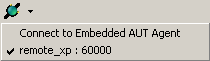
\includegraphics[width=0.60\textwidth]{52/ps/EmbeddedAgent}
\caption{Embedded AUT Agent}
\label{RNEmbeddedAgent}
\end{center}
\end{figure}


\end{itemize}


\textbf{Refactor: Replace with \gdcase{}}
\begin{itemize}
\item In the \gdtestcaseeditor{} and \gdtestsuiteeditor{}, there is a new option to replace one or more selected \gdcases{} with another \gdcase{} from the library. 
\item A new wizard takes you step-by-step through the replacement process, letting you transfer component names, match parameters and add further information for the new \gdcase{}.
\item This feature should help testers who want to restructure their tests after creating a reusable module to replace one or more \gdcases{}. 
\end{itemize}

\textbf{\gdomeditor{}: Cleanup unused component names}

\begin{itemize}
\item In the \gdomeditor{}, there is a new option in the context-sensitive menu. 
\item Via \bxmenu{Cleanup}{unused component names}{} \\
you can start a search for any component names that are no longer used in \gdsuites{} for this \gdaut{}. 
\item Once the search is finished, you can delete all of these unused names from the \gdomeditor{}. If they are then no longer used in the entire \gdproject{}, 
they can be deleted from the \gdcompnamebrowser{}. 

\begin{figure}[h]
\begin{center}
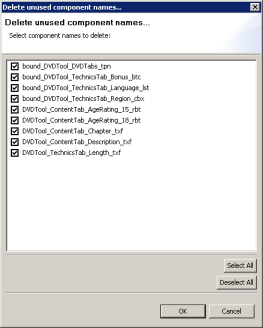
\includegraphics[width=0.60\textwidth]{52/ps/DeleteUnusedCompNames}
\caption{Deleting unused Component Names}
\label{RNDeleteUnusedCN}
\end{center}
\end{figure}
		
\end{itemize}

\textbf{HTML Test Result Reports can be expanded again}
\begin{itemize}
\item Following changes made for the initial contribution to Eclipse, the HTML Test Result Reports could not be viewed properly in the previous version. 
\item In this release, the nodes in the HTML reports can be expanded and collapsed to view the whole test progress. 

\begin{figure}[h]
\begin{center}
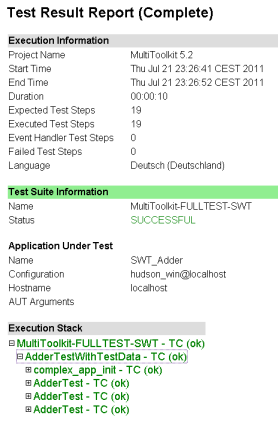
\includegraphics[width=0.60\textwidth]{52/ps/HTMLReport}
\caption{HTML Reports}
\label{RNHTMLReport}
\end{center}
\end{figure}
		
\end{itemize}

\textbf{State of component recognition displayed when collecting technical names}
\label{RNCompRec}
\begin{itemize}
\item When a component (technical name) is collected from an \gdaut{}, it receives a colored
dot corresponding to the accuracy of the object recognition for this component \textit{at the time of collecting}.
\begin{description}
\item [A green dot]{signifies that the component could be found with an exact match, and was the only component above the threshold}.
\item [A yellow dot]{means that the component is an exact match, but that multiple other components were also above the threshold.}
\item [A red dot]{ means that this component cannot be relocated in the current state of the \gdaut{}}
\end{description}
\item As a side effect, the colors on the component names (green) and technical names (red) that were displayed in previous versions are now no longer shown. Once the \gdomeditor{} has been saved, all names are shown with plain black icons. 
\begin{figure}[h]
\begin{center}
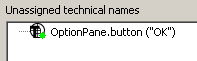
\includegraphics[width=0.6\textwidth]{52/ps/ColorDot}
\caption{Colored Dots for Object Mapping}
\label{RNColorDot}
\end{center}
\end{figure}
\end{itemize}

\textbf{Migration wizard re-enabled}
\begin{itemize}
\item  When migrating to the new version of \app{}, the migration assistant will automatically notify you that your database scheme is out-of-date. 
\item You can then select which \gdprojects{} to import (these must have been exported from the \gddb{} prior to migrating!).
\item The assistant will drop the tables in the \gddb{}, recreate the necessary tables and import the \gdprojects{} you specified.

\begin{figure}[h]
\begin{center}
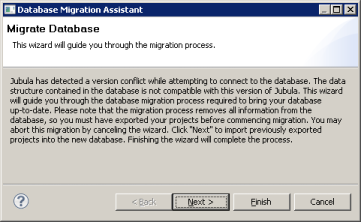
\includegraphics[width=0.6\textwidth]{52/ps/Migration}
\caption{Migration Wizard}
\label{RNMigration}
\end{center}
\end{figure}

\end{itemize}


\textbf{Copy ID to Clipboard also for \gdsuites{}}
\begin{itemize}
\item The ability to copy a unique ID to the clipboard to reference a \app{} element in external systems has also been implemented for \gdsuites{}. 
\item You can now copy the ID of a \gdcase{} or a \gdsuite{} to the clipboard, and also open an element based on its ID in the clipboard using \bxkey{Shift+F9}
\end{itemize}

\textbf{The DBTool is more verbose}
\begin{itemize}
\item The command line tool to import, export and delete \gdprojects{} in the \gddb{}, the DBTool, has been updated so that it is more verbose.
\end{itemize}

\textbf{Progress View}
\begin{itemize}
\item The \ite{} now  uses the progress view to show longer-running activities such as test execution, connecting to \gdauts{} etc.
\end{itemize}

\textbf{Edit Parameters Dialog in \gddataeditor{} can be opened via double-click}
\begin{itemize}
\item In the \gddataeditor{}  it is no longer necessary to open the Edit Parameters Dialog via context-menu, as it can now also be opened via double-click on the data set you wish to edit.
\end{itemize}


\textbf{Mac keyboards now supported, new mechanism for adding keyboard layout files}
\begin{itemize}
\item In the \gdaut{} configuration dialog for SWT and RCP \gdauts{}, the \bxname{Keyboard Layout} combo box now only offers 
layouts that have been defined for \app{}. German (DE) and English (US) are defined as standard. 
\item As well as being able to add keyboard layouts for other keyboards, you can also define platform-specific keyboard layouts (e.g. for Mac)
\item The documentation has been updated to describe the new mechanism for adding keyboard layouts.
\end{itemize}

\textbf{Object mapping: Degree of recognition accuracy for a test run can be viewed}
\begin{itemize}
\item The \gdomeditor{} has been extended so that the accuracy of component recognition is persisted and can be displayed.  
\item As well as displaying the state of component recognition when a technical name is collected from the \gdaut{} \bxpref{RNCompRec}, the degree of recognition accuracy is also noted 
for each test run. 
\item You can see the values for the recognition accuracy in two new BIRT reports in \app{}.
\begin{description}
\item [OMNameQuality]{shows a breakdown of the component names used in your test, and displays the degree of accuracy they were located during the test. You can use this report to see whether there are any component names that may need to be remapped (i.e. who are close to the threshold of not being found) before the test encounters a \bxname{Component Not Found} error. }
\item [OMNameQualityChart]{This report is a visual (graph) representation of the accuracy with which components were located during the test run. You can use the report to help you decide which components may need to be remapped, as they may soon result in a \bxname{Component Not Found} error during the test.}
\end{description}
\end{itemize}

\textbf{Mylyn: Refactored \gdcases{} are added to context}
\begin{itemize}
\item When working on a Mylyn task in app{}, \gdcases{} you create using the \bxname{refactor} function are now automatically added to the context.
\end{itemize}

\textbf{Mylyn: \gdcases{} opened via \bxkey{Ctrl+Shift+T} are added to context}
\begin{itemize}
\item When working on a Mylyn task in \app{}, \gdcases{} opened using the key combination \bxkey{Ctrl+Shift+T} are now automatically added to the context.
\end{itemize}

\textbf{Mylyn: \gdcases{} added via \gdcase{} reference dialog are added to context}
\begin{itemize}
\item When working on a Mylyn task in \app{}, \gdcases{} added using the \bxname{Add \gdcase{} reference} dialog are now automatically added to the context.
\end{itemize}

\textbf{Teststyle: Rules can now be viewed via the \gdpropview{}}
\begin{itemize}
\item When working with Teststyle, you can now open the \gdproject{} properties dialog to see the rule that has been flouted via:\\
\bxmenu{Show Teststyle Rule}{}{}\\
from the \gdprobview{}.
\end{itemize}

\textbf{Changes to BIRT reports}
\begin{itemize}
\item The BIRT report GUIdancerFULL has been removed.
\item There are new BIRT reports:
\begin{itemize}
\item \bxname{GUIdancerComments} shows a table of all failed relevant tests for the time specified, including the comment title that can be entered in the \gdtestsummaryview{}. This report is useful for delivering daily status reports of the tests.
\item \bxname{GUIdancerDuration} shows the duration of the chosen tests.
\item \bxname{GUIdancerExecutionHistogram} shows the proportion of executed, failed and non-executed \gdsteps{} for a test. This report is most useful when one specific \gdsuite{} is compared to see its progress over time. 
\item \bxname{TestresultSummary} shows a table of the \gdtestsummaryview{} for the dates and tests chosen. 
\end{itemize}
\item You can now also enter the \gdjob{} as a parameter for the report. The \gdsuites{} in the \gdjob{} are still displayed individually, however. 
\end{itemize}



\textbf{License Dialog: Restart prompt}
\begin{itemize}
\item Once a license has been added via the Preferences, a dialog is shown to remind you to restart \app{} before continuing. 
\item From the dialog you can choose to restart \app{} automatically.
\end{itemize}


\subsection{Known issues and other information}

\textbf{Problem displaying component names from browsers}
\begin{itemize}
\item In some siutations, when viewing the \gdcompnamesview{} from a browser, you may see GUIDs (a long number/character string) instead of the component name.
\item This is a problem displaying the component name at the moment and can be considered a display error, albeit a serious one. 
\item The component names themselves are correct, and can be seen either by opening the editor, or by refreshing the \gdproject{}.
\end{itemize}

\textbf{Issue with incorrect handling of \bxshell{null} in renderers fixed}
\begin{itemize}
\item Renderers in Swing that return \bxshell{null} can now be correctly handled.
\item See \url{http://eclip.se/426978} for more details. 
\end{itemize}

\textbf{Selenium update}
\begin{itemize}
\item We have updated the version of Selenium used for HTML tests to 2.39.
\end{itemize}

\textbf{Port number for embedded \gdagent{} changed}
\begin{itemize}
\item The default port number for the embedded \gdagent{} is now 60001.
\item You can change the default port number in the preferences.
\end{itemize}

\textbf{Table view has been removed from the \gdomeditor{}}
\begin{itemize}
\item The table view has been removed from the \gdomeditor{}.
\end{itemize}

\textbf{Problems opening BIRT reports when using IE11}
\begin{itemize}
\item There is a known issue with BIRT reporting that occurs when using Internet Explorer 11. 
\item There is a ticket open in the \gd{} Bugzilla (\url{https://bugzilla.bredex.de/show_bug.cgi?id=1281}) and in the Eclipse Bugzilla (\url{http://eclip.se/422056}) for this. The ticket in the Eclipse Bugzilla documents workarounds.
\end{itemize}

\textbf{Java 1.4 \gdauts{} no longer testable}
\begin{itemize}
\item As of this version, Java 1.4 \gdauts{} are no longer testable with the \ite{}. 
\end{itemize}

\textbf{Changes to the launcher for the \gdagent{}}
\begin{itemize}
\item The \gdagent{} is no longer available under the name \bxshell{autagent-lin} or \bxshell{autagent-sol}.
\item Use the launcher \bxshell{autagent} instead.
\end{itemize}

\textbf{Java 7 tests on Mac}
\begin{itemize}
\item There are still some issues running tests on Mac machines with Java 7. We suggest using Java 6 on Mac machines for the moment.
\end{itemize}

\textbf{Working directory for \ite{} and \gdagent{} on Linux}
\begin{itemize}
\item The \gdagent{} and the \ite{} now  use the current directory as their working directory on Linux systems.
\end{itemize}


\textbf{The \ite{} now uses Java 7}
\begin{itemize}
\item We have updated the version of Java installed with the \ite{} to version 7.
\end{itemize}

\textbf{The installer requires Java 7}
\begin{itemize}
\item You will need Java 7 installed to be able to run the installer.
\end{itemize}

\textbf{iOS 5.0 no longer supported}
\begin{itemize}
\item We no longer support testing on iOS 5.0 \gdauts{}.
\end{itemize}

\textbf{Working with RDP connections on Windows 8}
\begin{itemize}
\item Windows 8 users working with RDP connections for test execution should ensure that they have installed all updates for Windows. 
\end{itemize}

\textbf{Updated the version of EclipseLink used}
\begin{itemize}
\item In this version, we have switched to EclipseLink 2.5.1 and JPA 2.1.0.
\end{itemize}

\textbf{Vista support removed}
\begin{itemize}
\item We no longer execute tests on Vista: the support for Vista has been removed for this version.
\end{itemize}

\textbf{Multi-window mode for HTML testing on Mac OSX}
\begin{itemize}
\item There are known issues with starting \gdauts{} that are using the multi-window mode on Mac OSX, both in Firefox and Safari.
\item We have removed these combinations from our tests.
\end{itemize}

\textbf{Pure SWT \gdauts{} no longer tested}
\begin{itemize}
\item We no longer execute regression tests on pure SWT \gdauts{}. We do, however, perform various tests on RCP, which uses SWT components. 
\end{itemize}

\textbf{\gdagent{} started without console per default}
\begin{itemize}
\item The standalone \gdagent{} is now started without a console per default.
\item If you would like to see the console when starting the \gdagent{}, you must adapt the \bxname{autagent.ini} file.
\item In the -vm parameter, use \bxname{java} instead of \bxname{javaw}.
\end{itemize}


\section{Release Notes for \app{} version 6.0007x}

\subsection{New Features and Developments}

\textbf{Embedded gdagent{}}\\
\begin{itemize}
\item If you are starting your \gdaut{} and running your tests on your local machine, 
you can now connect to an embedded \gdagent{} directly from the \ite. 
\item This saves you having to start an \gdagent{} on localhost. 
\item This is also useful for testers working with \jb{} as a feature in an Eclipse installation. 
\item The embedded \gdagent{} is started on port 60000 by default; this number can be changed in the preferences.

\begin{figure}[h]
\begin{center}
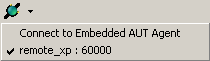
\includegraphics[width=0.60\textwidth]{52/ps/EmbeddedAgent}
\caption{Embedded AUT Agent}
\label{RNEmbeddedAgent}
\end{center}
\end{figure}


\end{itemize}


\textbf{Refactor: Replace with \gdcase{}}
\begin{itemize}
\item In the \gdtestcaseeditor{} and \gdtestsuiteeditor{}, there is a new option to replace one or more selected \gdcases{} with another \gdcase{} from the library. 
\item A new wizard takes you step-by-step through the replacement process, letting you transfer component names, match parameters and add further information for the new \gdcase{}.
\item This feature should help testers who want to restructure their tests after creating a reusable module to replace one or more \gdcases{}. 
\end{itemize}

\textbf{\gdomeditor{}: Cleanup unused component names}

\begin{itemize}
\item In the \gdomeditor{}, there is a new option in the context-sensitive menu. 
\item Via \bxmenu{Cleanup}{unused component names}{} \\
you can start a search for any component names that are no longer used in \gdsuites{} for this \gdaut{}. 
\item Once the search is finished, you can delete all of these unused names from the \gdomeditor{}. If they are then no longer used in the entire \gdproject{}, 
they can be deleted from the \gdcompnamebrowser{}. 

\begin{figure}[h]
\begin{center}
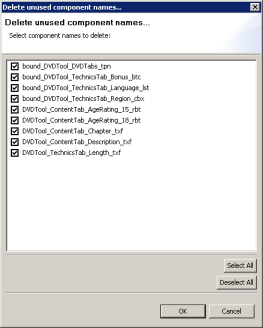
\includegraphics[width=0.60\textwidth]{52/ps/DeleteUnusedCompNames}
\caption{Deleting unused Component Names}
\label{RNDeleteUnusedCN}
\end{center}
\end{figure}
		
\end{itemize}

\textbf{HTML Test Result Reports can be expanded again}
\begin{itemize}
\item Following changes made for the initial contribution to Eclipse, the HTML Test Result Reports could not be viewed properly in the previous version. 
\item In this release, the nodes in the HTML reports can be expanded and collapsed to view the whole test progress. 

\begin{figure}[h]
\begin{center}
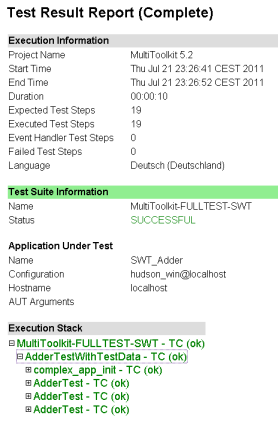
\includegraphics[width=0.60\textwidth]{52/ps/HTMLReport}
\caption{HTML Reports}
\label{RNHTMLReport}
\end{center}
\end{figure}
		
\end{itemize}

\textbf{State of component recognition displayed when collecting technical names}
\label{RNCompRec}
\begin{itemize}
\item When a component (technical name) is collected from an \gdaut{}, it receives a colored
dot corresponding to the accuracy of the object recognition for this component \textit{at the time of collecting}.
\begin{description}
\item [A green dot]{signifies that the component could be found with an exact match, and was the only component above the threshold}.
\item [A yellow dot]{means that the component is an exact match, but that multiple other components were also above the threshold.}
\item [A red dot]{ means that this component cannot be relocated in the current state of the \gdaut{}}
\end{description}
\item As a side effect, the colors on the component names (green) and technical names (red) that were displayed in previous versions are now no longer shown. Once the \gdomeditor{} has been saved, all names are shown with plain black icons. 
\begin{figure}[h]
\begin{center}
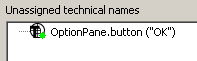
\includegraphics[width=0.6\textwidth]{52/ps/ColorDot}
\caption{Colored Dots for Object Mapping}
\label{RNColorDot}
\end{center}
\end{figure}
\end{itemize}

\textbf{Migration wizard re-enabled}
\begin{itemize}
\item  When migrating to the new version of \app{}, the migration assistant will automatically notify you that your database scheme is out-of-date. 
\item You can then select which \gdprojects{} to import (these must have been exported from the \gddb{} prior to migrating!).
\item The assistant will drop the tables in the \gddb{}, recreate the necessary tables and import the \gdprojects{} you specified.

\begin{figure}[h]
\begin{center}
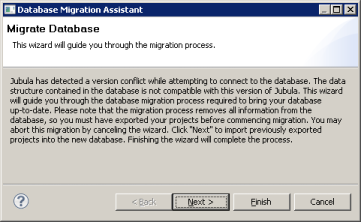
\includegraphics[width=0.6\textwidth]{52/ps/Migration}
\caption{Migration Wizard}
\label{RNMigration}
\end{center}
\end{figure}

\end{itemize}


\textbf{Copy ID to Clipboard also for \gdsuites{}}
\begin{itemize}
\item The ability to copy a unique ID to the clipboard to reference a \app{} element in external systems has also been implemented for \gdsuites{}. 
\item You can now copy the ID of a \gdcase{} or a \gdsuite{} to the clipboard, and also open an element based on its ID in the clipboard using \bxkey{Shift+F9}
\end{itemize}

\textbf{The DBTool is more verbose}
\begin{itemize}
\item The command line tool to import, export and delete \gdprojects{} in the \gddb{}, the DBTool, has been updated so that it is more verbose.
\end{itemize}

\textbf{Progress View}
\begin{itemize}
\item The \ite{} now  uses the progress view to show longer-running activities such as test execution, connecting to \gdauts{} etc.
\end{itemize}

\textbf{Edit Parameters Dialog in \gddataeditor{} can be opened via double-click}
\begin{itemize}
\item In the \gddataeditor{}  it is no longer necessary to open the Edit Parameters Dialog via context-menu, as it can now also be opened via double-click on the data set you wish to edit.
\end{itemize}


\textbf{Mac keyboards now supported, new mechanism for adding keyboard layout files}
\begin{itemize}
\item In the \gdaut{} configuration dialog for SWT and RCP \gdauts{}, the \bxname{Keyboard Layout} combo box now only offers 
layouts that have been defined for \app{}. German (DE) and English (US) are defined as standard. 
\item As well as being able to add keyboard layouts for other keyboards, you can also define platform-specific keyboard layouts (e.g. for Mac)
\item The documentation has been updated to describe the new mechanism for adding keyboard layouts.
\end{itemize}

\textbf{Object mapping: Degree of recognition accuracy for a test run can be viewed}
\begin{itemize}
\item The \gdomeditor{} has been extended so that the accuracy of component recognition is persisted and can be displayed.  
\item As well as displaying the state of component recognition when a technical name is collected from the \gdaut{} \bxpref{RNCompRec}, the degree of recognition accuracy is also noted 
for each test run. 
\item You can see the values for the recognition accuracy in two new BIRT reports in \app{}.
\begin{description}
\item [OMNameQuality]{shows a breakdown of the component names used in your test, and displays the degree of accuracy they were located during the test. You can use this report to see whether there are any component names that may need to be remapped (i.e. who are close to the threshold of not being found) before the test encounters a \bxname{Component Not Found} error. }
\item [OMNameQualityChart]{This report is a visual (graph) representation of the accuracy with which components were located during the test run. You can use the report to help you decide which components may need to be remapped, as they may soon result in a \bxname{Component Not Found} error during the test.}
\end{description}
\end{itemize}

\textbf{Mylyn: Refactored \gdcases{} are added to context}
\begin{itemize}
\item When working on a Mylyn task in app{}, \gdcases{} you create using the \bxname{refactor} function are now automatically added to the context.
\end{itemize}

\textbf{Mylyn: \gdcases{} opened via \bxkey{Ctrl+Shift+T} are added to context}
\begin{itemize}
\item When working on a Mylyn task in \app{}, \gdcases{} opened using the key combination \bxkey{Ctrl+Shift+T} are now automatically added to the context.
\end{itemize}

\textbf{Mylyn: \gdcases{} added via \gdcase{} reference dialog are added to context}
\begin{itemize}
\item When working on a Mylyn task in \app{}, \gdcases{} added using the \bxname{Add \gdcase{} reference} dialog are now automatically added to the context.
\end{itemize}

\textbf{Teststyle: Rules can now be viewed via the \gdpropview{}}
\begin{itemize}
\item When working with Teststyle, you can now open the \gdproject{} properties dialog to see the rule that has been flouted via:\\
\bxmenu{Show Teststyle Rule}{}{}\\
from the \gdprobview{}.
\end{itemize}

\textbf{Changes to BIRT reports}
\begin{itemize}
\item The BIRT report GUIdancerFULL has been removed.
\item There are new BIRT reports:
\begin{itemize}
\item \bxname{GUIdancerComments} shows a table of all failed relevant tests for the time specified, including the comment title that can be entered in the \gdtestsummaryview{}. This report is useful for delivering daily status reports of the tests.
\item \bxname{GUIdancerDuration} shows the duration of the chosen tests.
\item \bxname{GUIdancerExecutionHistogram} shows the proportion of executed, failed and non-executed \gdsteps{} for a test. This report is most useful when one specific \gdsuite{} is compared to see its progress over time. 
\item \bxname{TestresultSummary} shows a table of the \gdtestsummaryview{} for the dates and tests chosen. 
\end{itemize}
\item You can now also enter the \gdjob{} as a parameter for the report. The \gdsuites{} in the \gdjob{} are still displayed individually, however. 
\end{itemize}



\textbf{License Dialog: Restart prompt}
\begin{itemize}
\item Once a license has been added via the Preferences, a dialog is shown to remind you to restart \app{} before continuing. 
\item From the dialog you can choose to restart \app{} automatically.
\end{itemize}


\subsection{Known issues and other information}

\textbf{Problem displaying component names from browsers}
\begin{itemize}
\item In some siutations, when viewing the \gdcompnamesview{} from a browser, you may see GUIDs (a long number/character string) instead of the component name.
\item This is a problem displaying the component name at the moment and can be considered a display error, albeit a serious one. 
\item The component names themselves are correct, and can be seen either by opening the editor, or by refreshing the \gdproject{}.
\end{itemize}

\textbf{Issue with incorrect handling of \bxshell{null} in renderers fixed}
\begin{itemize}
\item Renderers in Swing that return \bxshell{null} can now be correctly handled.
\item See \url{http://eclip.se/426978} for more details. 
\end{itemize}

\textbf{Selenium update}
\begin{itemize}
\item We have updated the version of Selenium used for HTML tests to 2.39.
\end{itemize}

\textbf{Port number for embedded \gdagent{} changed}
\begin{itemize}
\item The default port number for the embedded \gdagent{} is now 60001.
\item You can change the default port number in the preferences.
\end{itemize}

\textbf{Table view has been removed from the \gdomeditor{}}
\begin{itemize}
\item The table view has been removed from the \gdomeditor{}.
\end{itemize}

\textbf{Problems opening BIRT reports when using IE11}
\begin{itemize}
\item There is a known issue with BIRT reporting that occurs when using Internet Explorer 11. 
\item There is a ticket open in the \gd{} Bugzilla (\url{https://bugzilla.bredex.de/show_bug.cgi?id=1281}) and in the Eclipse Bugzilla (\url{http://eclip.se/422056}) for this. The ticket in the Eclipse Bugzilla documents workarounds.
\end{itemize}

\textbf{Java 1.4 \gdauts{} no longer testable}
\begin{itemize}
\item As of this version, Java 1.4 \gdauts{} are no longer testable with the \ite{}. 
\end{itemize}

\textbf{Changes to the launcher for the \gdagent{}}
\begin{itemize}
\item The \gdagent{} is no longer available under the name \bxshell{autagent-lin} or \bxshell{autagent-sol}.
\item Use the launcher \bxshell{autagent} instead.
\end{itemize}

\textbf{Java 7 tests on Mac}
\begin{itemize}
\item There are still some issues running tests on Mac machines with Java 7. We suggest using Java 6 on Mac machines for the moment.
\end{itemize}

\textbf{Working directory for \ite{} and \gdagent{} on Linux}
\begin{itemize}
\item The \gdagent{} and the \ite{} now  use the current directory as their working directory on Linux systems.
\end{itemize}


\textbf{The \ite{} now uses Java 7}
\begin{itemize}
\item We have updated the version of Java installed with the \ite{} to version 7.
\end{itemize}

\textbf{The installer requires Java 7}
\begin{itemize}
\item You will need Java 7 installed to be able to run the installer.
\end{itemize}

\textbf{iOS 5.0 no longer supported}
\begin{itemize}
\item We no longer support testing on iOS 5.0 \gdauts{}.
\end{itemize}

\textbf{Working with RDP connections on Windows 8}
\begin{itemize}
\item Windows 8 users working with RDP connections for test execution should ensure that they have installed all updates for Windows. 
\end{itemize}

\textbf{Updated the version of EclipseLink used}
\begin{itemize}
\item In this version, we have switched to EclipseLink 2.5.1 and JPA 2.1.0.
\end{itemize}

\textbf{Vista support removed}
\begin{itemize}
\item We no longer execute tests on Vista: the support for Vista has been removed for this version.
\end{itemize}

\textbf{Multi-window mode for HTML testing on Mac OSX}
\begin{itemize}
\item There are known issues with starting \gdauts{} that are using the multi-window mode on Mac OSX, both in Firefox and Safari.
\item We have removed these combinations from our tests.
\end{itemize}

\textbf{Pure SWT \gdauts{} no longer tested}
\begin{itemize}
\item We no longer execute regression tests on pure SWT \gdauts{}. We do, however, perform various tests on RCP, which uses SWT components. 
\end{itemize}

\textbf{\gdagent{} started without console per default}
\begin{itemize}
\item The standalone \gdagent{} is now started without a console per default.
\item If you would like to see the console when starting the \gdagent{}, you must adapt the \bxname{autagent.ini} file.
\item In the -vm parameter, use \bxname{java} instead of \bxname{javaw}.
\end{itemize}


\section{Release Notes for \app{} version 6.0007x}

\subsection{New Features and Developments}

\textbf{Embedded gdagent{}}\\
\begin{itemize}
\item If you are starting your \gdaut{} and running your tests on your local machine, 
you can now connect to an embedded \gdagent{} directly from the \ite. 
\item This saves you having to start an \gdagent{} on localhost. 
\item This is also useful for testers working with \jb{} as a feature in an Eclipse installation. 
\item The embedded \gdagent{} is started on port 60000 by default; this number can be changed in the preferences.

\begin{figure}[h]
\begin{center}
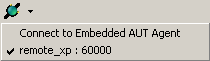
\includegraphics[width=0.60\textwidth]{52/ps/EmbeddedAgent}
\caption{Embedded AUT Agent}
\label{RNEmbeddedAgent}
\end{center}
\end{figure}


\end{itemize}


\textbf{Refactor: Replace with \gdcase{}}
\begin{itemize}
\item In the \gdtestcaseeditor{} and \gdtestsuiteeditor{}, there is a new option to replace one or more selected \gdcases{} with another \gdcase{} from the library. 
\item A new wizard takes you step-by-step through the replacement process, letting you transfer component names, match parameters and add further information for the new \gdcase{}.
\item This feature should help testers who want to restructure their tests after creating a reusable module to replace one or more \gdcases{}. 
\end{itemize}

\textbf{\gdomeditor{}: Cleanup unused component names}

\begin{itemize}
\item In the \gdomeditor{}, there is a new option in the context-sensitive menu. 
\item Via \bxmenu{Cleanup}{unused component names}{} \\
you can start a search for any component names that are no longer used in \gdsuites{} for this \gdaut{}. 
\item Once the search is finished, you can delete all of these unused names from the \gdomeditor{}. If they are then no longer used in the entire \gdproject{}, 
they can be deleted from the \gdcompnamebrowser{}. 

\begin{figure}[h]
\begin{center}
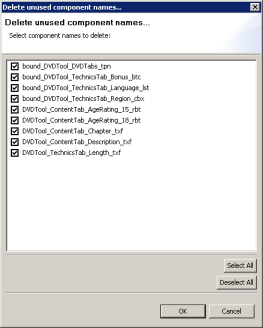
\includegraphics[width=0.60\textwidth]{52/ps/DeleteUnusedCompNames}
\caption{Deleting unused Component Names}
\label{RNDeleteUnusedCN}
\end{center}
\end{figure}
		
\end{itemize}

\textbf{HTML Test Result Reports can be expanded again}
\begin{itemize}
\item Following changes made for the initial contribution to Eclipse, the HTML Test Result Reports could not be viewed properly in the previous version. 
\item In this release, the nodes in the HTML reports can be expanded and collapsed to view the whole test progress. 

\begin{figure}[h]
\begin{center}
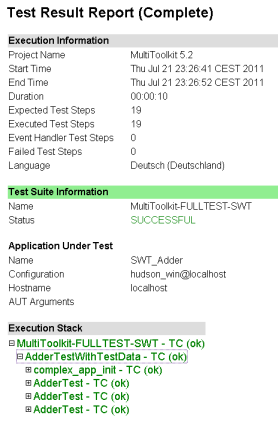
\includegraphics[width=0.60\textwidth]{52/ps/HTMLReport}
\caption{HTML Reports}
\label{RNHTMLReport}
\end{center}
\end{figure}
		
\end{itemize}

\textbf{State of component recognition displayed when collecting technical names}
\label{RNCompRec}
\begin{itemize}
\item When a component (technical name) is collected from an \gdaut{}, it receives a colored
dot corresponding to the accuracy of the object recognition for this component \textit{at the time of collecting}.
\begin{description}
\item [A green dot]{signifies that the component could be found with an exact match, and was the only component above the threshold}.
\item [A yellow dot]{means that the component is an exact match, but that multiple other components were also above the threshold.}
\item [A red dot]{ means that this component cannot be relocated in the current state of the \gdaut{}}
\end{description}
\item As a side effect, the colors on the component names (green) and technical names (red) that were displayed in previous versions are now no longer shown. Once the \gdomeditor{} has been saved, all names are shown with plain black icons. 
\begin{figure}[h]
\begin{center}
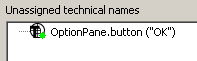
\includegraphics[width=0.6\textwidth]{52/ps/ColorDot}
\caption{Colored Dots for Object Mapping}
\label{RNColorDot}
\end{center}
\end{figure}
\end{itemize}

\textbf{Migration wizard re-enabled}
\begin{itemize}
\item  When migrating to the new version of \app{}, the migration assistant will automatically notify you that your database scheme is out-of-date. 
\item You can then select which \gdprojects{} to import (these must have been exported from the \gddb{} prior to migrating!).
\item The assistant will drop the tables in the \gddb{}, recreate the necessary tables and import the \gdprojects{} you specified.

\begin{figure}[h]
\begin{center}
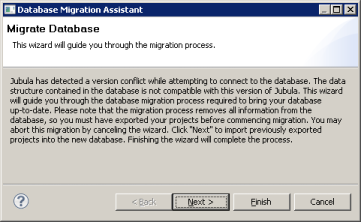
\includegraphics[width=0.6\textwidth]{52/ps/Migration}
\caption{Migration Wizard}
\label{RNMigration}
\end{center}
\end{figure}

\end{itemize}


\textbf{Copy ID to Clipboard also for \gdsuites{}}
\begin{itemize}
\item The ability to copy a unique ID to the clipboard to reference a \app{} element in external systems has also been implemented for \gdsuites{}. 
\item You can now copy the ID of a \gdcase{} or a \gdsuite{} to the clipboard, and also open an element based on its ID in the clipboard using \bxkey{Shift+F9}
\end{itemize}

\textbf{The DBTool is more verbose}
\begin{itemize}
\item The command line tool to import, export and delete \gdprojects{} in the \gddb{}, the DBTool, has been updated so that it is more verbose.
\end{itemize}

\textbf{Progress View}
\begin{itemize}
\item The \ite{} now  uses the progress view to show longer-running activities such as test execution, connecting to \gdauts{} etc.
\end{itemize}

\textbf{Edit Parameters Dialog in \gddataeditor{} can be opened via double-click}
\begin{itemize}
\item In the \gddataeditor{}  it is no longer necessary to open the Edit Parameters Dialog via context-menu, as it can now also be opened via double-click on the data set you wish to edit.
\end{itemize}


\textbf{Mac keyboards now supported, new mechanism for adding keyboard layout files}
\begin{itemize}
\item In the \gdaut{} configuration dialog for SWT and RCP \gdauts{}, the \bxname{Keyboard Layout} combo box now only offers 
layouts that have been defined for \app{}. German (DE) and English (US) are defined as standard. 
\item As well as being able to add keyboard layouts for other keyboards, you can also define platform-specific keyboard layouts (e.g. for Mac)
\item The documentation has been updated to describe the new mechanism for adding keyboard layouts.
\end{itemize}

\textbf{Object mapping: Degree of recognition accuracy for a test run can be viewed}
\begin{itemize}
\item The \gdomeditor{} has been extended so that the accuracy of component recognition is persisted and can be displayed.  
\item As well as displaying the state of component recognition when a technical name is collected from the \gdaut{} \bxpref{RNCompRec}, the degree of recognition accuracy is also noted 
for each test run. 
\item You can see the values for the recognition accuracy in two new BIRT reports in \app{}.
\begin{description}
\item [OMNameQuality]{shows a breakdown of the component names used in your test, and displays the degree of accuracy they were located during the test. You can use this report to see whether there are any component names that may need to be remapped (i.e. who are close to the threshold of not being found) before the test encounters a \bxname{Component Not Found} error. }
\item [OMNameQualityChart]{This report is a visual (graph) representation of the accuracy with which components were located during the test run. You can use the report to help you decide which components may need to be remapped, as they may soon result in a \bxname{Component Not Found} error during the test.}
\end{description}
\end{itemize}

\textbf{Mylyn: Refactored \gdcases{} are added to context}
\begin{itemize}
\item When working on a Mylyn task in app{}, \gdcases{} you create using the \bxname{refactor} function are now automatically added to the context.
\end{itemize}

\textbf{Mylyn: \gdcases{} opened via \bxkey{Ctrl+Shift+T} are added to context}
\begin{itemize}
\item When working on a Mylyn task in \app{}, \gdcases{} opened using the key combination \bxkey{Ctrl+Shift+T} are now automatically added to the context.
\end{itemize}

\textbf{Mylyn: \gdcases{} added via \gdcase{} reference dialog are added to context}
\begin{itemize}
\item When working on a Mylyn task in \app{}, \gdcases{} added using the \bxname{Add \gdcase{} reference} dialog are now automatically added to the context.
\end{itemize}

\textbf{Teststyle: Rules can now be viewed via the \gdpropview{}}
\begin{itemize}
\item When working with Teststyle, you can now open the \gdproject{} properties dialog to see the rule that has been flouted via:\\
\bxmenu{Show Teststyle Rule}{}{}\\
from the \gdprobview{}.
\end{itemize}

\textbf{Changes to BIRT reports}
\begin{itemize}
\item The BIRT report GUIdancerFULL has been removed.
\item There are new BIRT reports:
\begin{itemize}
\item \bxname{GUIdancerComments} shows a table of all failed relevant tests for the time specified, including the comment title that can be entered in the \gdtestsummaryview{}. This report is useful for delivering daily status reports of the tests.
\item \bxname{GUIdancerDuration} shows the duration of the chosen tests.
\item \bxname{GUIdancerExecutionHistogram} shows the proportion of executed, failed and non-executed \gdsteps{} for a test. This report is most useful when one specific \gdsuite{} is compared to see its progress over time. 
\item \bxname{TestresultSummary} shows a table of the \gdtestsummaryview{} for the dates and tests chosen. 
\end{itemize}
\item You can now also enter the \gdjob{} as a parameter for the report. The \gdsuites{} in the \gdjob{} are still displayed individually, however. 
\end{itemize}



\textbf{License Dialog: Restart prompt}
\begin{itemize}
\item Once a license has been added via the Preferences, a dialog is shown to remind you to restart \app{} before continuing. 
\item From the dialog you can choose to restart \app{} automatically.
\end{itemize}


\subsection{Known issues and other information}

\textbf{Problem displaying component names from browsers}
\begin{itemize}
\item In some siutations, when viewing the \gdcompnamesview{} from a browser, you may see GUIDs (a long number/character string) instead of the component name.
\item This is a problem displaying the component name at the moment and can be considered a display error, albeit a serious one. 
\item The component names themselves are correct, and can be seen either by opening the editor, or by refreshing the \gdproject{}.
\end{itemize}

\textbf{Issue with incorrect handling of \bxshell{null} in renderers fixed}
\begin{itemize}
\item Renderers in Swing that return \bxshell{null} can now be correctly handled.
\item See \url{http://eclip.se/426978} for more details. 
\end{itemize}

\textbf{Selenium update}
\begin{itemize}
\item We have updated the version of Selenium used for HTML tests to 2.39.
\end{itemize}

\textbf{Port number for embedded \gdagent{} changed}
\begin{itemize}
\item The default port number for the embedded \gdagent{} is now 60001.
\item You can change the default port number in the preferences.
\end{itemize}

\textbf{Table view has been removed from the \gdomeditor{}}
\begin{itemize}
\item The table view has been removed from the \gdomeditor{}.
\end{itemize}

\textbf{Problems opening BIRT reports when using IE11}
\begin{itemize}
\item There is a known issue with BIRT reporting that occurs when using Internet Explorer 11. 
\item There is a ticket open in the \gd{} Bugzilla (\url{https://bugzilla.bredex.de/show_bug.cgi?id=1281}) and in the Eclipse Bugzilla (\url{http://eclip.se/422056}) for this. The ticket in the Eclipse Bugzilla documents workarounds.
\end{itemize}

\textbf{Java 1.4 \gdauts{} no longer testable}
\begin{itemize}
\item As of this version, Java 1.4 \gdauts{} are no longer testable with the \ite{}. 
\end{itemize}

\textbf{Changes to the launcher for the \gdagent{}}
\begin{itemize}
\item The \gdagent{} is no longer available under the name \bxshell{autagent-lin} or \bxshell{autagent-sol}.
\item Use the launcher \bxshell{autagent} instead.
\end{itemize}

\textbf{Java 7 tests on Mac}
\begin{itemize}
\item There are still some issues running tests on Mac machines with Java 7. We suggest using Java 6 on Mac machines for the moment.
\end{itemize}

\textbf{Working directory for \ite{} and \gdagent{} on Linux}
\begin{itemize}
\item The \gdagent{} and the \ite{} now  use the current directory as their working directory on Linux systems.
\end{itemize}


\textbf{The \ite{} now uses Java 7}
\begin{itemize}
\item We have updated the version of Java installed with the \ite{} to version 7.
\end{itemize}

\textbf{The installer requires Java 7}
\begin{itemize}
\item You will need Java 7 installed to be able to run the installer.
\end{itemize}

\textbf{iOS 5.0 no longer supported}
\begin{itemize}
\item We no longer support testing on iOS 5.0 \gdauts{}.
\end{itemize}

\textbf{Working with RDP connections on Windows 8}
\begin{itemize}
\item Windows 8 users working with RDP connections for test execution should ensure that they have installed all updates for Windows. 
\end{itemize}

\textbf{Updated the version of EclipseLink used}
\begin{itemize}
\item In this version, we have switched to EclipseLink 2.5.1 and JPA 2.1.0.
\end{itemize}

\textbf{Vista support removed}
\begin{itemize}
\item We no longer execute tests on Vista: the support for Vista has been removed for this version.
\end{itemize}

\textbf{Multi-window mode for HTML testing on Mac OSX}
\begin{itemize}
\item There are known issues with starting \gdauts{} that are using the multi-window mode on Mac OSX, both in Firefox and Safari.
\item We have removed these combinations from our tests.
\end{itemize}

\textbf{Pure SWT \gdauts{} no longer tested}
\begin{itemize}
\item We no longer execute regression tests on pure SWT \gdauts{}. We do, however, perform various tests on RCP, which uses SWT components. 
\end{itemize}

\textbf{\gdagent{} started without console per default}
\begin{itemize}
\item The standalone \gdagent{} is now started without a console per default.
\item If you would like to see the console when starting the \gdagent{}, you must adapt the \bxname{autagent.ini} file.
\item In the -vm parameter, use \bxname{java} instead of \bxname{javaw}.
\end{itemize}


\section{Release Notes for \app{} version 6.0007x}

\subsection{New Features and Developments}

\textbf{Embedded gdagent{}}\\
\begin{itemize}
\item If you are starting your \gdaut{} and running your tests on your local machine, 
you can now connect to an embedded \gdagent{} directly from the \ite. 
\item This saves you having to start an \gdagent{} on localhost. 
\item This is also useful for testers working with \jb{} as a feature in an Eclipse installation. 
\item The embedded \gdagent{} is started on port 60000 by default; this number can be changed in the preferences.

\begin{figure}[h]
\begin{center}
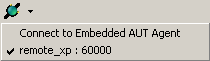
\includegraphics[width=0.60\textwidth]{52/ps/EmbeddedAgent}
\caption{Embedded AUT Agent}
\label{RNEmbeddedAgent}
\end{center}
\end{figure}


\end{itemize}


\textbf{Refactor: Replace with \gdcase{}}
\begin{itemize}
\item In the \gdtestcaseeditor{} and \gdtestsuiteeditor{}, there is a new option to replace one or more selected \gdcases{} with another \gdcase{} from the library. 
\item A new wizard takes you step-by-step through the replacement process, letting you transfer component names, match parameters and add further information for the new \gdcase{}.
\item This feature should help testers who want to restructure their tests after creating a reusable module to replace one or more \gdcases{}. 
\end{itemize}

\textbf{\gdomeditor{}: Cleanup unused component names}

\begin{itemize}
\item In the \gdomeditor{}, there is a new option in the context-sensitive menu. 
\item Via \bxmenu{Cleanup}{unused component names}{} \\
you can start a search for any component names that are no longer used in \gdsuites{} for this \gdaut{}. 
\item Once the search is finished, you can delete all of these unused names from the \gdomeditor{}. If they are then no longer used in the entire \gdproject{}, 
they can be deleted from the \gdcompnamebrowser{}. 

\begin{figure}[h]
\begin{center}
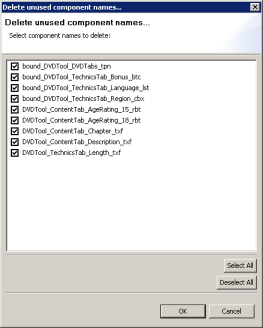
\includegraphics[width=0.60\textwidth]{52/ps/DeleteUnusedCompNames}
\caption{Deleting unused Component Names}
\label{RNDeleteUnusedCN}
\end{center}
\end{figure}
		
\end{itemize}

\textbf{HTML Test Result Reports can be expanded again}
\begin{itemize}
\item Following changes made for the initial contribution to Eclipse, the HTML Test Result Reports could not be viewed properly in the previous version. 
\item In this release, the nodes in the HTML reports can be expanded and collapsed to view the whole test progress. 

\begin{figure}[h]
\begin{center}
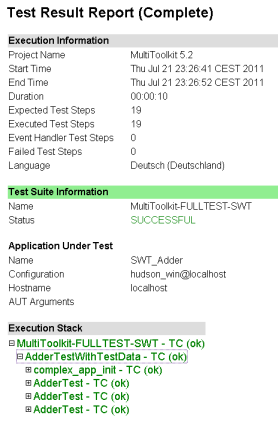
\includegraphics[width=0.60\textwidth]{52/ps/HTMLReport}
\caption{HTML Reports}
\label{RNHTMLReport}
\end{center}
\end{figure}
		
\end{itemize}

\textbf{State of component recognition displayed when collecting technical names}
\label{RNCompRec}
\begin{itemize}
\item When a component (technical name) is collected from an \gdaut{}, it receives a colored
dot corresponding to the accuracy of the object recognition for this component \textit{at the time of collecting}.
\begin{description}
\item [A green dot]{signifies that the component could be found with an exact match, and was the only component above the threshold}.
\item [A yellow dot]{means that the component is an exact match, but that multiple other components were also above the threshold.}
\item [A red dot]{ means that this component cannot be relocated in the current state of the \gdaut{}}
\end{description}
\item As a side effect, the colors on the component names (green) and technical names (red) that were displayed in previous versions are now no longer shown. Once the \gdomeditor{} has been saved, all names are shown with plain black icons. 
\begin{figure}[h]
\begin{center}
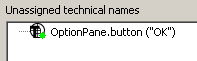
\includegraphics[width=0.6\textwidth]{52/ps/ColorDot}
\caption{Colored Dots for Object Mapping}
\label{RNColorDot}
\end{center}
\end{figure}
\end{itemize}

\textbf{Migration wizard re-enabled}
\begin{itemize}
\item  When migrating to the new version of \app{}, the migration assistant will automatically notify you that your database scheme is out-of-date. 
\item You can then select which \gdprojects{} to import (these must have been exported from the \gddb{} prior to migrating!).
\item The assistant will drop the tables in the \gddb{}, recreate the necessary tables and import the \gdprojects{} you specified.

\begin{figure}[h]
\begin{center}
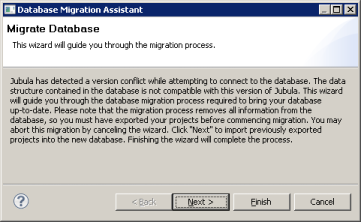
\includegraphics[width=0.6\textwidth]{52/ps/Migration}
\caption{Migration Wizard}
\label{RNMigration}
\end{center}
\end{figure}

\end{itemize}


\textbf{Copy ID to Clipboard also for \gdsuites{}}
\begin{itemize}
\item The ability to copy a unique ID to the clipboard to reference a \app{} element in external systems has also been implemented for \gdsuites{}. 
\item You can now copy the ID of a \gdcase{} or a \gdsuite{} to the clipboard, and also open an element based on its ID in the clipboard using \bxkey{Shift+F9}
\end{itemize}

\textbf{The DBTool is more verbose}
\begin{itemize}
\item The command line tool to import, export and delete \gdprojects{} in the \gddb{}, the DBTool, has been updated so that it is more verbose.
\end{itemize}

\textbf{Progress View}
\begin{itemize}
\item The \ite{} now  uses the progress view to show longer-running activities such as test execution, connecting to \gdauts{} etc.
\end{itemize}

\textbf{Edit Parameters Dialog in \gddataeditor{} can be opened via double-click}
\begin{itemize}
\item In the \gddataeditor{}  it is no longer necessary to open the Edit Parameters Dialog via context-menu, as it can now also be opened via double-click on the data set you wish to edit.
\end{itemize}


\textbf{Mac keyboards now supported, new mechanism for adding keyboard layout files}
\begin{itemize}
\item In the \gdaut{} configuration dialog for SWT and RCP \gdauts{}, the \bxname{Keyboard Layout} combo box now only offers 
layouts that have been defined for \app{}. German (DE) and English (US) are defined as standard. 
\item As well as being able to add keyboard layouts for other keyboards, you can also define platform-specific keyboard layouts (e.g. for Mac)
\item The documentation has been updated to describe the new mechanism for adding keyboard layouts.
\end{itemize}

\textbf{Object mapping: Degree of recognition accuracy for a test run can be viewed}
\begin{itemize}
\item The \gdomeditor{} has been extended so that the accuracy of component recognition is persisted and can be displayed.  
\item As well as displaying the state of component recognition when a technical name is collected from the \gdaut{} \bxpref{RNCompRec}, the degree of recognition accuracy is also noted 
for each test run. 
\item You can see the values for the recognition accuracy in two new BIRT reports in \app{}.
\begin{description}
\item [OMNameQuality]{shows a breakdown of the component names used in your test, and displays the degree of accuracy they were located during the test. You can use this report to see whether there are any component names that may need to be remapped (i.e. who are close to the threshold of not being found) before the test encounters a \bxname{Component Not Found} error. }
\item [OMNameQualityChart]{This report is a visual (graph) representation of the accuracy with which components were located during the test run. You can use the report to help you decide which components may need to be remapped, as they may soon result in a \bxname{Component Not Found} error during the test.}
\end{description}
\end{itemize}

\textbf{Mylyn: Refactored \gdcases{} are added to context}
\begin{itemize}
\item When working on a Mylyn task in app{}, \gdcases{} you create using the \bxname{refactor} function are now automatically added to the context.
\end{itemize}

\textbf{Mylyn: \gdcases{} opened via \bxkey{Ctrl+Shift+T} are added to context}
\begin{itemize}
\item When working on a Mylyn task in \app{}, \gdcases{} opened using the key combination \bxkey{Ctrl+Shift+T} are now automatically added to the context.
\end{itemize}

\textbf{Mylyn: \gdcases{} added via \gdcase{} reference dialog are added to context}
\begin{itemize}
\item When working on a Mylyn task in \app{}, \gdcases{} added using the \bxname{Add \gdcase{} reference} dialog are now automatically added to the context.
\end{itemize}

\textbf{Teststyle: Rules can now be viewed via the \gdpropview{}}
\begin{itemize}
\item When working with Teststyle, you can now open the \gdproject{} properties dialog to see the rule that has been flouted via:\\
\bxmenu{Show Teststyle Rule}{}{}\\
from the \gdprobview{}.
\end{itemize}

\textbf{Changes to BIRT reports}
\begin{itemize}
\item The BIRT report GUIdancerFULL has been removed.
\item There are new BIRT reports:
\begin{itemize}
\item \bxname{GUIdancerComments} shows a table of all failed relevant tests for the time specified, including the comment title that can be entered in the \gdtestsummaryview{}. This report is useful for delivering daily status reports of the tests.
\item \bxname{GUIdancerDuration} shows the duration of the chosen tests.
\item \bxname{GUIdancerExecutionHistogram} shows the proportion of executed, failed and non-executed \gdsteps{} for a test. This report is most useful when one specific \gdsuite{} is compared to see its progress over time. 
\item \bxname{TestresultSummary} shows a table of the \gdtestsummaryview{} for the dates and tests chosen. 
\end{itemize}
\item You can now also enter the \gdjob{} as a parameter for the report. The \gdsuites{} in the \gdjob{} are still displayed individually, however. 
\end{itemize}



\textbf{License Dialog: Restart prompt}
\begin{itemize}
\item Once a license has been added via the Preferences, a dialog is shown to remind you to restart \app{} before continuing. 
\item From the dialog you can choose to restart \app{} automatically.
\end{itemize}


\subsection{Known issues and other information}

\textbf{Problem displaying component names from browsers}
\begin{itemize}
\item In some siutations, when viewing the \gdcompnamesview{} from a browser, you may see GUIDs (a long number/character string) instead of the component name.
\item This is a problem displaying the component name at the moment and can be considered a display error, albeit a serious one. 
\item The component names themselves are correct, and can be seen either by opening the editor, or by refreshing the \gdproject{}.
\end{itemize}

\textbf{Issue with incorrect handling of \bxshell{null} in renderers fixed}
\begin{itemize}
\item Renderers in Swing that return \bxshell{null} can now be correctly handled.
\item See \url{http://eclip.se/426978} for more details. 
\end{itemize}

\textbf{Selenium update}
\begin{itemize}
\item We have updated the version of Selenium used for HTML tests to 2.39.
\end{itemize}

\textbf{Port number for embedded \gdagent{} changed}
\begin{itemize}
\item The default port number for the embedded \gdagent{} is now 60001.
\item You can change the default port number in the preferences.
\end{itemize}

\textbf{Table view has been removed from the \gdomeditor{}}
\begin{itemize}
\item The table view has been removed from the \gdomeditor{}.
\end{itemize}

\textbf{Problems opening BIRT reports when using IE11}
\begin{itemize}
\item There is a known issue with BIRT reporting that occurs when using Internet Explorer 11. 
\item There is a ticket open in the \gd{} Bugzilla (\url{https://bugzilla.bredex.de/show_bug.cgi?id=1281}) and in the Eclipse Bugzilla (\url{http://eclip.se/422056}) for this. The ticket in the Eclipse Bugzilla documents workarounds.
\end{itemize}

\textbf{Java 1.4 \gdauts{} no longer testable}
\begin{itemize}
\item As of this version, Java 1.4 \gdauts{} are no longer testable with the \ite{}. 
\end{itemize}

\textbf{Changes to the launcher for the \gdagent{}}
\begin{itemize}
\item The \gdagent{} is no longer available under the name \bxshell{autagent-lin} or \bxshell{autagent-sol}.
\item Use the launcher \bxshell{autagent} instead.
\end{itemize}

\textbf{Java 7 tests on Mac}
\begin{itemize}
\item There are still some issues running tests on Mac machines with Java 7. We suggest using Java 6 on Mac machines for the moment.
\end{itemize}

\textbf{Working directory for \ite{} and \gdagent{} on Linux}
\begin{itemize}
\item The \gdagent{} and the \ite{} now  use the current directory as their working directory on Linux systems.
\end{itemize}


\textbf{The \ite{} now uses Java 7}
\begin{itemize}
\item We have updated the version of Java installed with the \ite{} to version 7.
\end{itemize}

\textbf{The installer requires Java 7}
\begin{itemize}
\item You will need Java 7 installed to be able to run the installer.
\end{itemize}

\textbf{iOS 5.0 no longer supported}
\begin{itemize}
\item We no longer support testing on iOS 5.0 \gdauts{}.
\end{itemize}

\textbf{Working with RDP connections on Windows 8}
\begin{itemize}
\item Windows 8 users working with RDP connections for test execution should ensure that they have installed all updates for Windows. 
\end{itemize}

\textbf{Updated the version of EclipseLink used}
\begin{itemize}
\item In this version, we have switched to EclipseLink 2.5.1 and JPA 2.1.0.
\end{itemize}

\textbf{Vista support removed}
\begin{itemize}
\item We no longer execute tests on Vista: the support for Vista has been removed for this version.
\end{itemize}

\textbf{Multi-window mode for HTML testing on Mac OSX}
\begin{itemize}
\item There are known issues with starting \gdauts{} that are using the multi-window mode on Mac OSX, both in Firefox and Safari.
\item We have removed these combinations from our tests.
\end{itemize}

\textbf{Pure SWT \gdauts{} no longer tested}
\begin{itemize}
\item We no longer execute regression tests on pure SWT \gdauts{}. We do, however, perform various tests on RCP, which uses SWT components. 
\end{itemize}

\textbf{\gdagent{} started without console per default}
\begin{itemize}
\item The standalone \gdagent{} is now started without a console per default.
\item If you would like to see the console when starting the \gdagent{}, you must adapt the \bxname{autagent.ini} file.
\item In the -vm parameter, use \bxname{java} instead of \bxname{javaw}.
\end{itemize}


\section{Release Notes for \app{} version 6.0007x}

\subsection{New Features and Developments}

\textbf{Embedded gdagent{}}\\
\begin{itemize}
\item If you are starting your \gdaut{} and running your tests on your local machine, 
you can now connect to an embedded \gdagent{} directly from the \ite. 
\item This saves you having to start an \gdagent{} on localhost. 
\item This is also useful for testers working with \jb{} as a feature in an Eclipse installation. 
\item The embedded \gdagent{} is started on port 60000 by default; this number can be changed in the preferences.

\begin{figure}[h]
\begin{center}
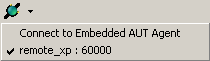
\includegraphics[width=0.60\textwidth]{52/ps/EmbeddedAgent}
\caption{Embedded AUT Agent}
\label{RNEmbeddedAgent}
\end{center}
\end{figure}


\end{itemize}


\textbf{Refactor: Replace with \gdcase{}}
\begin{itemize}
\item In the \gdtestcaseeditor{} and \gdtestsuiteeditor{}, there is a new option to replace one or more selected \gdcases{} with another \gdcase{} from the library. 
\item A new wizard takes you step-by-step through the replacement process, letting you transfer component names, match parameters and add further information for the new \gdcase{}.
\item This feature should help testers who want to restructure their tests after creating a reusable module to replace one or more \gdcases{}. 
\end{itemize}

\textbf{\gdomeditor{}: Cleanup unused component names}

\begin{itemize}
\item In the \gdomeditor{}, there is a new option in the context-sensitive menu. 
\item Via \bxmenu{Cleanup}{unused component names}{} \\
you can start a search for any component names that are no longer used in \gdsuites{} for this \gdaut{}. 
\item Once the search is finished, you can delete all of these unused names from the \gdomeditor{}. If they are then no longer used in the entire \gdproject{}, 
they can be deleted from the \gdcompnamebrowser{}. 

\begin{figure}[h]
\begin{center}
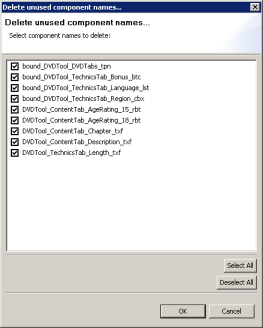
\includegraphics[width=0.60\textwidth]{52/ps/DeleteUnusedCompNames}
\caption{Deleting unused Component Names}
\label{RNDeleteUnusedCN}
\end{center}
\end{figure}
		
\end{itemize}

\textbf{HTML Test Result Reports can be expanded again}
\begin{itemize}
\item Following changes made for the initial contribution to Eclipse, the HTML Test Result Reports could not be viewed properly in the previous version. 
\item In this release, the nodes in the HTML reports can be expanded and collapsed to view the whole test progress. 

\begin{figure}[h]
\begin{center}
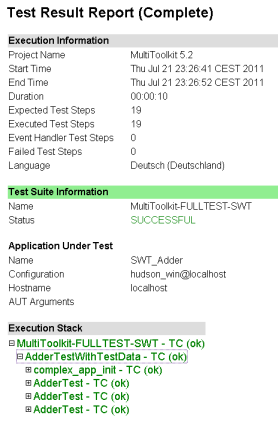
\includegraphics[width=0.60\textwidth]{52/ps/HTMLReport}
\caption{HTML Reports}
\label{RNHTMLReport}
\end{center}
\end{figure}
		
\end{itemize}

\textbf{State of component recognition displayed when collecting technical names}
\label{RNCompRec}
\begin{itemize}
\item When a component (technical name) is collected from an \gdaut{}, it receives a colored
dot corresponding to the accuracy of the object recognition for this component \textit{at the time of collecting}.
\begin{description}
\item [A green dot]{signifies that the component could be found with an exact match, and was the only component above the threshold}.
\item [A yellow dot]{means that the component is an exact match, but that multiple other components were also above the threshold.}
\item [A red dot]{ means that this component cannot be relocated in the current state of the \gdaut{}}
\end{description}
\item As a side effect, the colors on the component names (green) and technical names (red) that were displayed in previous versions are now no longer shown. Once the \gdomeditor{} has been saved, all names are shown with plain black icons. 
\begin{figure}[h]
\begin{center}
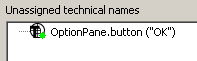
\includegraphics[width=0.6\textwidth]{52/ps/ColorDot}
\caption{Colored Dots for Object Mapping}
\label{RNColorDot}
\end{center}
\end{figure}
\end{itemize}

\textbf{Migration wizard re-enabled}
\begin{itemize}
\item  When migrating to the new version of \app{}, the migration assistant will automatically notify you that your database scheme is out-of-date. 
\item You can then select which \gdprojects{} to import (these must have been exported from the \gddb{} prior to migrating!).
\item The assistant will drop the tables in the \gddb{}, recreate the necessary tables and import the \gdprojects{} you specified.

\begin{figure}[h]
\begin{center}
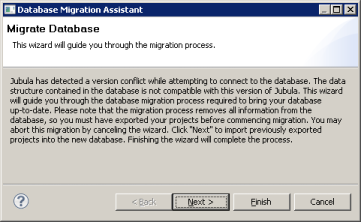
\includegraphics[width=0.6\textwidth]{52/ps/Migration}
\caption{Migration Wizard}
\label{RNMigration}
\end{center}
\end{figure}

\end{itemize}


\textbf{Copy ID to Clipboard also for \gdsuites{}}
\begin{itemize}
\item The ability to copy a unique ID to the clipboard to reference a \app{} element in external systems has also been implemented for \gdsuites{}. 
\item You can now copy the ID of a \gdcase{} or a \gdsuite{} to the clipboard, and also open an element based on its ID in the clipboard using \bxkey{Shift+F9}
\end{itemize}

\textbf{The DBTool is more verbose}
\begin{itemize}
\item The command line tool to import, export and delete \gdprojects{} in the \gddb{}, the DBTool, has been updated so that it is more verbose.
\end{itemize}

\textbf{Progress View}
\begin{itemize}
\item The \ite{} now  uses the progress view to show longer-running activities such as test execution, connecting to \gdauts{} etc.
\end{itemize}

\textbf{Edit Parameters Dialog in \gddataeditor{} can be opened via double-click}
\begin{itemize}
\item In the \gddataeditor{}  it is no longer necessary to open the Edit Parameters Dialog via context-menu, as it can now also be opened via double-click on the data set you wish to edit.
\end{itemize}


\textbf{Mac keyboards now supported, new mechanism for adding keyboard layout files}
\begin{itemize}
\item In the \gdaut{} configuration dialog for SWT and RCP \gdauts{}, the \bxname{Keyboard Layout} combo box now only offers 
layouts that have been defined for \app{}. German (DE) and English (US) are defined as standard. 
\item As well as being able to add keyboard layouts for other keyboards, you can also define platform-specific keyboard layouts (e.g. for Mac)
\item The documentation has been updated to describe the new mechanism for adding keyboard layouts.
\end{itemize}

\textbf{Object mapping: Degree of recognition accuracy for a test run can be viewed}
\begin{itemize}
\item The \gdomeditor{} has been extended so that the accuracy of component recognition is persisted and can be displayed.  
\item As well as displaying the state of component recognition when a technical name is collected from the \gdaut{} \bxpref{RNCompRec}, the degree of recognition accuracy is also noted 
for each test run. 
\item You can see the values for the recognition accuracy in two new BIRT reports in \app{}.
\begin{description}
\item [OMNameQuality]{shows a breakdown of the component names used in your test, and displays the degree of accuracy they were located during the test. You can use this report to see whether there are any component names that may need to be remapped (i.e. who are close to the threshold of not being found) before the test encounters a \bxname{Component Not Found} error. }
\item [OMNameQualityChart]{This report is a visual (graph) representation of the accuracy with which components were located during the test run. You can use the report to help you decide which components may need to be remapped, as they may soon result in a \bxname{Component Not Found} error during the test.}
\end{description}
\end{itemize}

\textbf{Mylyn: Refactored \gdcases{} are added to context}
\begin{itemize}
\item When working on a Mylyn task in app{}, \gdcases{} you create using the \bxname{refactor} function are now automatically added to the context.
\end{itemize}

\textbf{Mylyn: \gdcases{} opened via \bxkey{Ctrl+Shift+T} are added to context}
\begin{itemize}
\item When working on a Mylyn task in \app{}, \gdcases{} opened using the key combination \bxkey{Ctrl+Shift+T} are now automatically added to the context.
\end{itemize}

\textbf{Mylyn: \gdcases{} added via \gdcase{} reference dialog are added to context}
\begin{itemize}
\item When working on a Mylyn task in \app{}, \gdcases{} added using the \bxname{Add \gdcase{} reference} dialog are now automatically added to the context.
\end{itemize}

\textbf{Teststyle: Rules can now be viewed via the \gdpropview{}}
\begin{itemize}
\item When working with Teststyle, you can now open the \gdproject{} properties dialog to see the rule that has been flouted via:\\
\bxmenu{Show Teststyle Rule}{}{}\\
from the \gdprobview{}.
\end{itemize}

\textbf{Changes to BIRT reports}
\begin{itemize}
\item The BIRT report GUIdancerFULL has been removed.
\item There are new BIRT reports:
\begin{itemize}
\item \bxname{GUIdancerComments} shows a table of all failed relevant tests for the time specified, including the comment title that can be entered in the \gdtestsummaryview{}. This report is useful for delivering daily status reports of the tests.
\item \bxname{GUIdancerDuration} shows the duration of the chosen tests.
\item \bxname{GUIdancerExecutionHistogram} shows the proportion of executed, failed and non-executed \gdsteps{} for a test. This report is most useful when one specific \gdsuite{} is compared to see its progress over time. 
\item \bxname{TestresultSummary} shows a table of the \gdtestsummaryview{} for the dates and tests chosen. 
\end{itemize}
\item You can now also enter the \gdjob{} as a parameter for the report. The \gdsuites{} in the \gdjob{} are still displayed individually, however. 
\end{itemize}



\textbf{License Dialog: Restart prompt}
\begin{itemize}
\item Once a license has been added via the Preferences, a dialog is shown to remind you to restart \app{} before continuing. 
\item From the dialog you can choose to restart \app{} automatically.
\end{itemize}


\subsection{Known issues and other information}

\textbf{Problem displaying component names from browsers}
\begin{itemize}
\item In some siutations, when viewing the \gdcompnamesview{} from a browser, you may see GUIDs (a long number/character string) instead of the component name.
\item This is a problem displaying the component name at the moment and can be considered a display error, albeit a serious one. 
\item The component names themselves are correct, and can be seen either by opening the editor, or by refreshing the \gdproject{}.
\end{itemize}

\textbf{Issue with incorrect handling of \bxshell{null} in renderers fixed}
\begin{itemize}
\item Renderers in Swing that return \bxshell{null} can now be correctly handled.
\item See \url{http://eclip.se/426978} for more details. 
\end{itemize}

\textbf{Selenium update}
\begin{itemize}
\item We have updated the version of Selenium used for HTML tests to 2.39.
\end{itemize}

\textbf{Port number for embedded \gdagent{} changed}
\begin{itemize}
\item The default port number for the embedded \gdagent{} is now 60001.
\item You can change the default port number in the preferences.
\end{itemize}

\textbf{Table view has been removed from the \gdomeditor{}}
\begin{itemize}
\item The table view has been removed from the \gdomeditor{}.
\end{itemize}

\textbf{Problems opening BIRT reports when using IE11}
\begin{itemize}
\item There is a known issue with BIRT reporting that occurs when using Internet Explorer 11. 
\item There is a ticket open in the \gd{} Bugzilla (\url{https://bugzilla.bredex.de/show_bug.cgi?id=1281}) and in the Eclipse Bugzilla (\url{http://eclip.se/422056}) for this. The ticket in the Eclipse Bugzilla documents workarounds.
\end{itemize}

\textbf{Java 1.4 \gdauts{} no longer testable}
\begin{itemize}
\item As of this version, Java 1.4 \gdauts{} are no longer testable with the \ite{}. 
\end{itemize}

\textbf{Changes to the launcher for the \gdagent{}}
\begin{itemize}
\item The \gdagent{} is no longer available under the name \bxshell{autagent-lin} or \bxshell{autagent-sol}.
\item Use the launcher \bxshell{autagent} instead.
\end{itemize}

\textbf{Java 7 tests on Mac}
\begin{itemize}
\item There are still some issues running tests on Mac machines with Java 7. We suggest using Java 6 on Mac machines for the moment.
\end{itemize}

\textbf{Working directory for \ite{} and \gdagent{} on Linux}
\begin{itemize}
\item The \gdagent{} and the \ite{} now  use the current directory as their working directory on Linux systems.
\end{itemize}


\textbf{The \ite{} now uses Java 7}
\begin{itemize}
\item We have updated the version of Java installed with the \ite{} to version 7.
\end{itemize}

\textbf{The installer requires Java 7}
\begin{itemize}
\item You will need Java 7 installed to be able to run the installer.
\end{itemize}

\textbf{iOS 5.0 no longer supported}
\begin{itemize}
\item We no longer support testing on iOS 5.0 \gdauts{}.
\end{itemize}

\textbf{Working with RDP connections on Windows 8}
\begin{itemize}
\item Windows 8 users working with RDP connections for test execution should ensure that they have installed all updates for Windows. 
\end{itemize}

\textbf{Updated the version of EclipseLink used}
\begin{itemize}
\item In this version, we have switched to EclipseLink 2.5.1 and JPA 2.1.0.
\end{itemize}

\textbf{Vista support removed}
\begin{itemize}
\item We no longer execute tests on Vista: the support for Vista has been removed for this version.
\end{itemize}

\textbf{Multi-window mode for HTML testing on Mac OSX}
\begin{itemize}
\item There are known issues with starting \gdauts{} that are using the multi-window mode on Mac OSX, both in Firefox and Safari.
\item We have removed these combinations from our tests.
\end{itemize}

\textbf{Pure SWT \gdauts{} no longer tested}
\begin{itemize}
\item We no longer execute regression tests on pure SWT \gdauts{}. We do, however, perform various tests on RCP, which uses SWT components. 
\end{itemize}

\textbf{\gdagent{} started without console per default}
\begin{itemize}
\item The standalone \gdagent{} is now started without a console per default.
\item If you would like to see the console when starting the \gdagent{}, you must adapt the \bxname{autagent.ini} file.
\item In the -vm parameter, use \bxname{java} instead of \bxname{javaw}.
\end{itemize}


\section{Release Notes for \app{} version 6.0007x}

\subsection{New Features and Developments}

\textbf{Embedded gdagent{}}\\
\begin{itemize}
\item If you are starting your \gdaut{} and running your tests on your local machine, 
you can now connect to an embedded \gdagent{} directly from the \ite. 
\item This saves you having to start an \gdagent{} on localhost. 
\item This is also useful for testers working with \jb{} as a feature in an Eclipse installation. 
\item The embedded \gdagent{} is started on port 60000 by default; this number can be changed in the preferences.

\begin{figure}[h]
\begin{center}
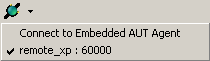
\includegraphics[width=0.60\textwidth]{52/ps/EmbeddedAgent}
\caption{Embedded AUT Agent}
\label{RNEmbeddedAgent}
\end{center}
\end{figure}


\end{itemize}


\textbf{Refactor: Replace with \gdcase{}}
\begin{itemize}
\item In the \gdtestcaseeditor{} and \gdtestsuiteeditor{}, there is a new option to replace one or more selected \gdcases{} with another \gdcase{} from the library. 
\item A new wizard takes you step-by-step through the replacement process, letting you transfer component names, match parameters and add further information for the new \gdcase{}.
\item This feature should help testers who want to restructure their tests after creating a reusable module to replace one or more \gdcases{}. 
\end{itemize}

\textbf{\gdomeditor{}: Cleanup unused component names}

\begin{itemize}
\item In the \gdomeditor{}, there is a new option in the context-sensitive menu. 
\item Via \bxmenu{Cleanup}{unused component names}{} \\
you can start a search for any component names that are no longer used in \gdsuites{} for this \gdaut{}. 
\item Once the search is finished, you can delete all of these unused names from the \gdomeditor{}. If they are then no longer used in the entire \gdproject{}, 
they can be deleted from the \gdcompnamebrowser{}. 

\begin{figure}[h]
\begin{center}
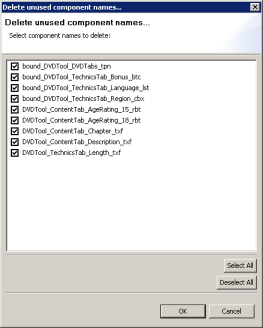
\includegraphics[width=0.60\textwidth]{52/ps/DeleteUnusedCompNames}
\caption{Deleting unused Component Names}
\label{RNDeleteUnusedCN}
\end{center}
\end{figure}
		
\end{itemize}

\textbf{HTML Test Result Reports can be expanded again}
\begin{itemize}
\item Following changes made for the initial contribution to Eclipse, the HTML Test Result Reports could not be viewed properly in the previous version. 
\item In this release, the nodes in the HTML reports can be expanded and collapsed to view the whole test progress. 

\begin{figure}[h]
\begin{center}
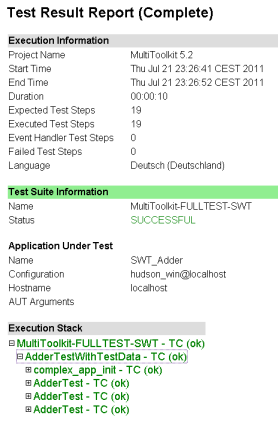
\includegraphics[width=0.60\textwidth]{52/ps/HTMLReport}
\caption{HTML Reports}
\label{RNHTMLReport}
\end{center}
\end{figure}
		
\end{itemize}

\textbf{State of component recognition displayed when collecting technical names}
\label{RNCompRec}
\begin{itemize}
\item When a component (technical name) is collected from an \gdaut{}, it receives a colored
dot corresponding to the accuracy of the object recognition for this component \textit{at the time of collecting}.
\begin{description}
\item [A green dot]{signifies that the component could be found with an exact match, and was the only component above the threshold}.
\item [A yellow dot]{means that the component is an exact match, but that multiple other components were also above the threshold.}
\item [A red dot]{ means that this component cannot be relocated in the current state of the \gdaut{}}
\end{description}
\item As a side effect, the colors on the component names (green) and technical names (red) that were displayed in previous versions are now no longer shown. Once the \gdomeditor{} has been saved, all names are shown with plain black icons. 
\begin{figure}[h]
\begin{center}
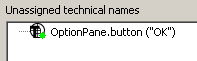
\includegraphics[width=0.6\textwidth]{52/ps/ColorDot}
\caption{Colored Dots for Object Mapping}
\label{RNColorDot}
\end{center}
\end{figure}
\end{itemize}

\textbf{Migration wizard re-enabled}
\begin{itemize}
\item  When migrating to the new version of \app{}, the migration assistant will automatically notify you that your database scheme is out-of-date. 
\item You can then select which \gdprojects{} to import (these must have been exported from the \gddb{} prior to migrating!).
\item The assistant will drop the tables in the \gddb{}, recreate the necessary tables and import the \gdprojects{} you specified.

\begin{figure}[h]
\begin{center}
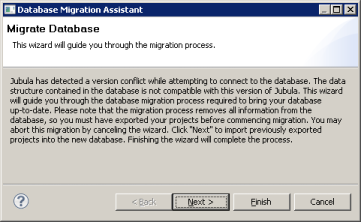
\includegraphics[width=0.6\textwidth]{52/ps/Migration}
\caption{Migration Wizard}
\label{RNMigration}
\end{center}
\end{figure}

\end{itemize}


\textbf{Copy ID to Clipboard also for \gdsuites{}}
\begin{itemize}
\item The ability to copy a unique ID to the clipboard to reference a \app{} element in external systems has also been implemented for \gdsuites{}. 
\item You can now copy the ID of a \gdcase{} or a \gdsuite{} to the clipboard, and also open an element based on its ID in the clipboard using \bxkey{Shift+F9}
\end{itemize}

\textbf{The DBTool is more verbose}
\begin{itemize}
\item The command line tool to import, export and delete \gdprojects{} in the \gddb{}, the DBTool, has been updated so that it is more verbose.
\end{itemize}

\textbf{Progress View}
\begin{itemize}
\item The \ite{} now  uses the progress view to show longer-running activities such as test execution, connecting to \gdauts{} etc.
\end{itemize}

\textbf{Edit Parameters Dialog in \gddataeditor{} can be opened via double-click}
\begin{itemize}
\item In the \gddataeditor{}  it is no longer necessary to open the Edit Parameters Dialog via context-menu, as it can now also be opened via double-click on the data set you wish to edit.
\end{itemize}


\textbf{Mac keyboards now supported, new mechanism for adding keyboard layout files}
\begin{itemize}
\item In the \gdaut{} configuration dialog for SWT and RCP \gdauts{}, the \bxname{Keyboard Layout} combo box now only offers 
layouts that have been defined for \app{}. German (DE) and English (US) are defined as standard. 
\item As well as being able to add keyboard layouts for other keyboards, you can also define platform-specific keyboard layouts (e.g. for Mac)
\item The documentation has been updated to describe the new mechanism for adding keyboard layouts.
\end{itemize}

\textbf{Object mapping: Degree of recognition accuracy for a test run can be viewed}
\begin{itemize}
\item The \gdomeditor{} has been extended so that the accuracy of component recognition is persisted and can be displayed.  
\item As well as displaying the state of component recognition when a technical name is collected from the \gdaut{} \bxpref{RNCompRec}, the degree of recognition accuracy is also noted 
for each test run. 
\item You can see the values for the recognition accuracy in two new BIRT reports in \app{}.
\begin{description}
\item [OMNameQuality]{shows a breakdown of the component names used in your test, and displays the degree of accuracy they were located during the test. You can use this report to see whether there are any component names that may need to be remapped (i.e. who are close to the threshold of not being found) before the test encounters a \bxname{Component Not Found} error. }
\item [OMNameQualityChart]{This report is a visual (graph) representation of the accuracy with which components were located during the test run. You can use the report to help you decide which components may need to be remapped, as they may soon result in a \bxname{Component Not Found} error during the test.}
\end{description}
\end{itemize}

\textbf{Mylyn: Refactored \gdcases{} are added to context}
\begin{itemize}
\item When working on a Mylyn task in app{}, \gdcases{} you create using the \bxname{refactor} function are now automatically added to the context.
\end{itemize}

\textbf{Mylyn: \gdcases{} opened via \bxkey{Ctrl+Shift+T} are added to context}
\begin{itemize}
\item When working on a Mylyn task in \app{}, \gdcases{} opened using the key combination \bxkey{Ctrl+Shift+T} are now automatically added to the context.
\end{itemize}

\textbf{Mylyn: \gdcases{} added via \gdcase{} reference dialog are added to context}
\begin{itemize}
\item When working on a Mylyn task in \app{}, \gdcases{} added using the \bxname{Add \gdcase{} reference} dialog are now automatically added to the context.
\end{itemize}

\textbf{Teststyle: Rules can now be viewed via the \gdpropview{}}
\begin{itemize}
\item When working with Teststyle, you can now open the \gdproject{} properties dialog to see the rule that has been flouted via:\\
\bxmenu{Show Teststyle Rule}{}{}\\
from the \gdprobview{}.
\end{itemize}

\textbf{Changes to BIRT reports}
\begin{itemize}
\item The BIRT report GUIdancerFULL has been removed.
\item There are new BIRT reports:
\begin{itemize}
\item \bxname{GUIdancerComments} shows a table of all failed relevant tests for the time specified, including the comment title that can be entered in the \gdtestsummaryview{}. This report is useful for delivering daily status reports of the tests.
\item \bxname{GUIdancerDuration} shows the duration of the chosen tests.
\item \bxname{GUIdancerExecutionHistogram} shows the proportion of executed, failed and non-executed \gdsteps{} for a test. This report is most useful when one specific \gdsuite{} is compared to see its progress over time. 
\item \bxname{TestresultSummary} shows a table of the \gdtestsummaryview{} for the dates and tests chosen. 
\end{itemize}
\item You can now also enter the \gdjob{} as a parameter for the report. The \gdsuites{} in the \gdjob{} are still displayed individually, however. 
\end{itemize}



\textbf{License Dialog: Restart prompt}
\begin{itemize}
\item Once a license has been added via the Preferences, a dialog is shown to remind you to restart \app{} before continuing. 
\item From the dialog you can choose to restart \app{} automatically.
\end{itemize}


\subsection{Known issues and other information}

\textbf{Problem displaying component names from browsers}
\begin{itemize}
\item In some siutations, when viewing the \gdcompnamesview{} from a browser, you may see GUIDs (a long number/character string) instead of the component name.
\item This is a problem displaying the component name at the moment and can be considered a display error, albeit a serious one. 
\item The component names themselves are correct, and can be seen either by opening the editor, or by refreshing the \gdproject{}.
\end{itemize}

\textbf{Issue with incorrect handling of \bxshell{null} in renderers fixed}
\begin{itemize}
\item Renderers in Swing that return \bxshell{null} can now be correctly handled.
\item See \url{http://eclip.se/426978} for more details. 
\end{itemize}

\textbf{Selenium update}
\begin{itemize}
\item We have updated the version of Selenium used for HTML tests to 2.39.
\end{itemize}

\textbf{Port number for embedded \gdagent{} changed}
\begin{itemize}
\item The default port number for the embedded \gdagent{} is now 60001.
\item You can change the default port number in the preferences.
\end{itemize}

\textbf{Table view has been removed from the \gdomeditor{}}
\begin{itemize}
\item The table view has been removed from the \gdomeditor{}.
\end{itemize}

\textbf{Problems opening BIRT reports when using IE11}
\begin{itemize}
\item There is a known issue with BIRT reporting that occurs when using Internet Explorer 11. 
\item There is a ticket open in the \gd{} Bugzilla (\url{https://bugzilla.bredex.de/show_bug.cgi?id=1281}) and in the Eclipse Bugzilla (\url{http://eclip.se/422056}) for this. The ticket in the Eclipse Bugzilla documents workarounds.
\end{itemize}

\textbf{Java 1.4 \gdauts{} no longer testable}
\begin{itemize}
\item As of this version, Java 1.4 \gdauts{} are no longer testable with the \ite{}. 
\end{itemize}

\textbf{Changes to the launcher for the \gdagent{}}
\begin{itemize}
\item The \gdagent{} is no longer available under the name \bxshell{autagent-lin} or \bxshell{autagent-sol}.
\item Use the launcher \bxshell{autagent} instead.
\end{itemize}

\textbf{Java 7 tests on Mac}
\begin{itemize}
\item There are still some issues running tests on Mac machines with Java 7. We suggest using Java 6 on Mac machines for the moment.
\end{itemize}

\textbf{Working directory for \ite{} and \gdagent{} on Linux}
\begin{itemize}
\item The \gdagent{} and the \ite{} now  use the current directory as their working directory on Linux systems.
\end{itemize}


\textbf{The \ite{} now uses Java 7}
\begin{itemize}
\item We have updated the version of Java installed with the \ite{} to version 7.
\end{itemize}

\textbf{The installer requires Java 7}
\begin{itemize}
\item You will need Java 7 installed to be able to run the installer.
\end{itemize}

\textbf{iOS 5.0 no longer supported}
\begin{itemize}
\item We no longer support testing on iOS 5.0 \gdauts{}.
\end{itemize}

\textbf{Working with RDP connections on Windows 8}
\begin{itemize}
\item Windows 8 users working with RDP connections for test execution should ensure that they have installed all updates for Windows. 
\end{itemize}

\textbf{Updated the version of EclipseLink used}
\begin{itemize}
\item In this version, we have switched to EclipseLink 2.5.1 and JPA 2.1.0.
\end{itemize}

\textbf{Vista support removed}
\begin{itemize}
\item We no longer execute tests on Vista: the support for Vista has been removed for this version.
\end{itemize}

\textbf{Multi-window mode for HTML testing on Mac OSX}
\begin{itemize}
\item There are known issues with starting \gdauts{} that are using the multi-window mode on Mac OSX, both in Firefox and Safari.
\item We have removed these combinations from our tests.
\end{itemize}

\textbf{Pure SWT \gdauts{} no longer tested}
\begin{itemize}
\item We no longer execute regression tests on pure SWT \gdauts{}. We do, however, perform various tests on RCP, which uses SWT components. 
\end{itemize}

\textbf{\gdagent{} started without console per default}
\begin{itemize}
\item The standalone \gdagent{} is now started without a console per default.
\item If you would like to see the console when starting the \gdagent{}, you must adapt the \bxname{autagent.ini} file.
\item In the -vm parameter, use \bxname{java} instead of \bxname{javaw}.
\end{itemize}


\section{Release Notes for \app{} version 6.0007x}

\subsection{New Features and Developments}

\textbf{Embedded gdagent{}}\\
\begin{itemize}
\item If you are starting your \gdaut{} and running your tests on your local machine, 
you can now connect to an embedded \gdagent{} directly from the \ite. 
\item This saves you having to start an \gdagent{} on localhost. 
\item This is also useful for testers working with \jb{} as a feature in an Eclipse installation. 
\item The embedded \gdagent{} is started on port 60000 by default; this number can be changed in the preferences.

\begin{figure}[h]
\begin{center}
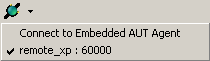
\includegraphics[width=0.60\textwidth]{52/ps/EmbeddedAgent}
\caption{Embedded AUT Agent}
\label{RNEmbeddedAgent}
\end{center}
\end{figure}


\end{itemize}


\textbf{Refactor: Replace with \gdcase{}}
\begin{itemize}
\item In the \gdtestcaseeditor{} and \gdtestsuiteeditor{}, there is a new option to replace one or more selected \gdcases{} with another \gdcase{} from the library. 
\item A new wizard takes you step-by-step through the replacement process, letting you transfer component names, match parameters and add further information for the new \gdcase{}.
\item This feature should help testers who want to restructure their tests after creating a reusable module to replace one or more \gdcases{}. 
\end{itemize}

\textbf{\gdomeditor{}: Cleanup unused component names}

\begin{itemize}
\item In the \gdomeditor{}, there is a new option in the context-sensitive menu. 
\item Via \bxmenu{Cleanup}{unused component names}{} \\
you can start a search for any component names that are no longer used in \gdsuites{} for this \gdaut{}. 
\item Once the search is finished, you can delete all of these unused names from the \gdomeditor{}. If they are then no longer used in the entire \gdproject{}, 
they can be deleted from the \gdcompnamebrowser{}. 

\begin{figure}[h]
\begin{center}
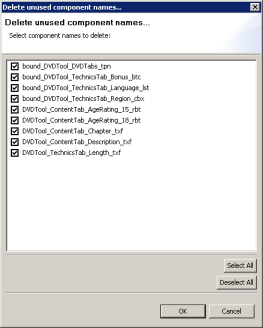
\includegraphics[width=0.60\textwidth]{52/ps/DeleteUnusedCompNames}
\caption{Deleting unused Component Names}
\label{RNDeleteUnusedCN}
\end{center}
\end{figure}
		
\end{itemize}

\textbf{HTML Test Result Reports can be expanded again}
\begin{itemize}
\item Following changes made for the initial contribution to Eclipse, the HTML Test Result Reports could not be viewed properly in the previous version. 
\item In this release, the nodes in the HTML reports can be expanded and collapsed to view the whole test progress. 

\begin{figure}[h]
\begin{center}
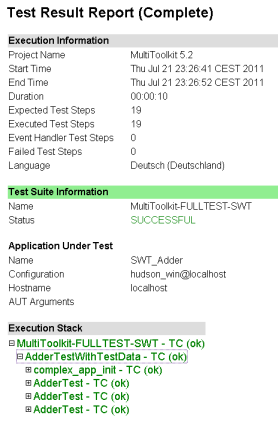
\includegraphics[width=0.60\textwidth]{52/ps/HTMLReport}
\caption{HTML Reports}
\label{RNHTMLReport}
\end{center}
\end{figure}
		
\end{itemize}

\textbf{State of component recognition displayed when collecting technical names}
\label{RNCompRec}
\begin{itemize}
\item When a component (technical name) is collected from an \gdaut{}, it receives a colored
dot corresponding to the accuracy of the object recognition for this component \textit{at the time of collecting}.
\begin{description}
\item [A green dot]{signifies that the component could be found with an exact match, and was the only component above the threshold}.
\item [A yellow dot]{means that the component is an exact match, but that multiple other components were also above the threshold.}
\item [A red dot]{ means that this component cannot be relocated in the current state of the \gdaut{}}
\end{description}
\item As a side effect, the colors on the component names (green) and technical names (red) that were displayed in previous versions are now no longer shown. Once the \gdomeditor{} has been saved, all names are shown with plain black icons. 
\begin{figure}[h]
\begin{center}
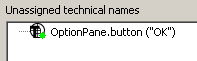
\includegraphics[width=0.6\textwidth]{52/ps/ColorDot}
\caption{Colored Dots for Object Mapping}
\label{RNColorDot}
\end{center}
\end{figure}
\end{itemize}

\textbf{Migration wizard re-enabled}
\begin{itemize}
\item  When migrating to the new version of \app{}, the migration assistant will automatically notify you that your database scheme is out-of-date. 
\item You can then select which \gdprojects{} to import (these must have been exported from the \gddb{} prior to migrating!).
\item The assistant will drop the tables in the \gddb{}, recreate the necessary tables and import the \gdprojects{} you specified.

\begin{figure}[h]
\begin{center}
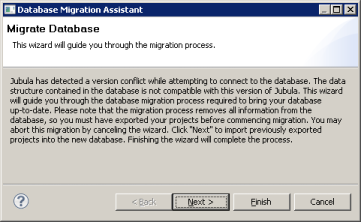
\includegraphics[width=0.6\textwidth]{52/ps/Migration}
\caption{Migration Wizard}
\label{RNMigration}
\end{center}
\end{figure}

\end{itemize}


\textbf{Copy ID to Clipboard also for \gdsuites{}}
\begin{itemize}
\item The ability to copy a unique ID to the clipboard to reference a \app{} element in external systems has also been implemented for \gdsuites{}. 
\item You can now copy the ID of a \gdcase{} or a \gdsuite{} to the clipboard, and also open an element based on its ID in the clipboard using \bxkey{Shift+F9}
\end{itemize}

\textbf{The DBTool is more verbose}
\begin{itemize}
\item The command line tool to import, export and delete \gdprojects{} in the \gddb{}, the DBTool, has been updated so that it is more verbose.
\end{itemize}

\textbf{Progress View}
\begin{itemize}
\item The \ite{} now  uses the progress view to show longer-running activities such as test execution, connecting to \gdauts{} etc.
\end{itemize}

\textbf{Edit Parameters Dialog in \gddataeditor{} can be opened via double-click}
\begin{itemize}
\item In the \gddataeditor{}  it is no longer necessary to open the Edit Parameters Dialog via context-menu, as it can now also be opened via double-click on the data set you wish to edit.
\end{itemize}


\textbf{Mac keyboards now supported, new mechanism for adding keyboard layout files}
\begin{itemize}
\item In the \gdaut{} configuration dialog for SWT and RCP \gdauts{}, the \bxname{Keyboard Layout} combo box now only offers 
layouts that have been defined for \app{}. German (DE) and English (US) are defined as standard. 
\item As well as being able to add keyboard layouts for other keyboards, you can also define platform-specific keyboard layouts (e.g. for Mac)
\item The documentation has been updated to describe the new mechanism for adding keyboard layouts.
\end{itemize}

\textbf{Object mapping: Degree of recognition accuracy for a test run can be viewed}
\begin{itemize}
\item The \gdomeditor{} has been extended so that the accuracy of component recognition is persisted and can be displayed.  
\item As well as displaying the state of component recognition when a technical name is collected from the \gdaut{} \bxpref{RNCompRec}, the degree of recognition accuracy is also noted 
for each test run. 
\item You can see the values for the recognition accuracy in two new BIRT reports in \app{}.
\begin{description}
\item [OMNameQuality]{shows a breakdown of the component names used in your test, and displays the degree of accuracy they were located during the test. You can use this report to see whether there are any component names that may need to be remapped (i.e. who are close to the threshold of not being found) before the test encounters a \bxname{Component Not Found} error. }
\item [OMNameQualityChart]{This report is a visual (graph) representation of the accuracy with which components were located during the test run. You can use the report to help you decide which components may need to be remapped, as they may soon result in a \bxname{Component Not Found} error during the test.}
\end{description}
\end{itemize}

\textbf{Mylyn: Refactored \gdcases{} are added to context}
\begin{itemize}
\item When working on a Mylyn task in app{}, \gdcases{} you create using the \bxname{refactor} function are now automatically added to the context.
\end{itemize}

\textbf{Mylyn: \gdcases{} opened via \bxkey{Ctrl+Shift+T} are added to context}
\begin{itemize}
\item When working on a Mylyn task in \app{}, \gdcases{} opened using the key combination \bxkey{Ctrl+Shift+T} are now automatically added to the context.
\end{itemize}

\textbf{Mylyn: \gdcases{} added via \gdcase{} reference dialog are added to context}
\begin{itemize}
\item When working on a Mylyn task in \app{}, \gdcases{} added using the \bxname{Add \gdcase{} reference} dialog are now automatically added to the context.
\end{itemize}

\textbf{Teststyle: Rules can now be viewed via the \gdpropview{}}
\begin{itemize}
\item When working with Teststyle, you can now open the \gdproject{} properties dialog to see the rule that has been flouted via:\\
\bxmenu{Show Teststyle Rule}{}{}\\
from the \gdprobview{}.
\end{itemize}

\textbf{Changes to BIRT reports}
\begin{itemize}
\item The BIRT report GUIdancerFULL has been removed.
\item There are new BIRT reports:
\begin{itemize}
\item \bxname{GUIdancerComments} shows a table of all failed relevant tests for the time specified, including the comment title that can be entered in the \gdtestsummaryview{}. This report is useful for delivering daily status reports of the tests.
\item \bxname{GUIdancerDuration} shows the duration of the chosen tests.
\item \bxname{GUIdancerExecutionHistogram} shows the proportion of executed, failed and non-executed \gdsteps{} for a test. This report is most useful when one specific \gdsuite{} is compared to see its progress over time. 
\item \bxname{TestresultSummary} shows a table of the \gdtestsummaryview{} for the dates and tests chosen. 
\end{itemize}
\item You can now also enter the \gdjob{} as a parameter for the report. The \gdsuites{} in the \gdjob{} are still displayed individually, however. 
\end{itemize}



\textbf{License Dialog: Restart prompt}
\begin{itemize}
\item Once a license has been added via the Preferences, a dialog is shown to remind you to restart \app{} before continuing. 
\item From the dialog you can choose to restart \app{} automatically.
\end{itemize}


\subsection{Known issues and other information}

\textbf{Problem displaying component names from browsers}
\begin{itemize}
\item In some siutations, when viewing the \gdcompnamesview{} from a browser, you may see GUIDs (a long number/character string) instead of the component name.
\item This is a problem displaying the component name at the moment and can be considered a display error, albeit a serious one. 
\item The component names themselves are correct, and can be seen either by opening the editor, or by refreshing the \gdproject{}.
\end{itemize}

\textbf{Issue with incorrect handling of \bxshell{null} in renderers fixed}
\begin{itemize}
\item Renderers in Swing that return \bxshell{null} can now be correctly handled.
\item See \url{http://eclip.se/426978} for more details. 
\end{itemize}

\textbf{Selenium update}
\begin{itemize}
\item We have updated the version of Selenium used for HTML tests to 2.39.
\end{itemize}

\textbf{Port number for embedded \gdagent{} changed}
\begin{itemize}
\item The default port number for the embedded \gdagent{} is now 60001.
\item You can change the default port number in the preferences.
\end{itemize}

\textbf{Table view has been removed from the \gdomeditor{}}
\begin{itemize}
\item The table view has been removed from the \gdomeditor{}.
\end{itemize}

\textbf{Problems opening BIRT reports when using IE11}
\begin{itemize}
\item There is a known issue with BIRT reporting that occurs when using Internet Explorer 11. 
\item There is a ticket open in the \gd{} Bugzilla (\url{https://bugzilla.bredex.de/show_bug.cgi?id=1281}) and in the Eclipse Bugzilla (\url{http://eclip.se/422056}) for this. The ticket in the Eclipse Bugzilla documents workarounds.
\end{itemize}

\textbf{Java 1.4 \gdauts{} no longer testable}
\begin{itemize}
\item As of this version, Java 1.4 \gdauts{} are no longer testable with the \ite{}. 
\end{itemize}

\textbf{Changes to the launcher for the \gdagent{}}
\begin{itemize}
\item The \gdagent{} is no longer available under the name \bxshell{autagent-lin} or \bxshell{autagent-sol}.
\item Use the launcher \bxshell{autagent} instead.
\end{itemize}

\textbf{Java 7 tests on Mac}
\begin{itemize}
\item There are still some issues running tests on Mac machines with Java 7. We suggest using Java 6 on Mac machines for the moment.
\end{itemize}

\textbf{Working directory for \ite{} and \gdagent{} on Linux}
\begin{itemize}
\item The \gdagent{} and the \ite{} now  use the current directory as their working directory on Linux systems.
\end{itemize}


\textbf{The \ite{} now uses Java 7}
\begin{itemize}
\item We have updated the version of Java installed with the \ite{} to version 7.
\end{itemize}

\textbf{The installer requires Java 7}
\begin{itemize}
\item You will need Java 7 installed to be able to run the installer.
\end{itemize}

\textbf{iOS 5.0 no longer supported}
\begin{itemize}
\item We no longer support testing on iOS 5.0 \gdauts{}.
\end{itemize}

\textbf{Working with RDP connections on Windows 8}
\begin{itemize}
\item Windows 8 users working with RDP connections for test execution should ensure that they have installed all updates for Windows. 
\end{itemize}

\textbf{Updated the version of EclipseLink used}
\begin{itemize}
\item In this version, we have switched to EclipseLink 2.5.1 and JPA 2.1.0.
\end{itemize}

\textbf{Vista support removed}
\begin{itemize}
\item We no longer execute tests on Vista: the support for Vista has been removed for this version.
\end{itemize}

\textbf{Multi-window mode for HTML testing on Mac OSX}
\begin{itemize}
\item There are known issues with starting \gdauts{} that are using the multi-window mode on Mac OSX, both in Firefox and Safari.
\item We have removed these combinations from our tests.
\end{itemize}

\textbf{Pure SWT \gdauts{} no longer tested}
\begin{itemize}
\item We no longer execute regression tests on pure SWT \gdauts{}. We do, however, perform various tests on RCP, which uses SWT components. 
\end{itemize}

\textbf{\gdagent{} started without console per default}
\begin{itemize}
\item The standalone \gdagent{} is now started without a console per default.
\item If you would like to see the console when starting the \gdagent{}, you must adapt the \bxname{autagent.ini} file.
\item In the -vm parameter, use \bxname{java} instead of \bxname{javaw}.
\end{itemize}


\section{Release Notes for \app{} version 6.0007x}

\subsection{New Features and Developments}

\textbf{Embedded gdagent{}}\\
\begin{itemize}
\item If you are starting your \gdaut{} and running your tests on your local machine, 
you can now connect to an embedded \gdagent{} directly from the \ite. 
\item This saves you having to start an \gdagent{} on localhost. 
\item This is also useful for testers working with \jb{} as a feature in an Eclipse installation. 
\item The embedded \gdagent{} is started on port 60000 by default; this number can be changed in the preferences.

\begin{figure}[h]
\begin{center}
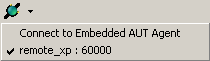
\includegraphics[width=0.60\textwidth]{52/ps/EmbeddedAgent}
\caption{Embedded AUT Agent}
\label{RNEmbeddedAgent}
\end{center}
\end{figure}


\end{itemize}


\textbf{Refactor: Replace with \gdcase{}}
\begin{itemize}
\item In the \gdtestcaseeditor{} and \gdtestsuiteeditor{}, there is a new option to replace one or more selected \gdcases{} with another \gdcase{} from the library. 
\item A new wizard takes you step-by-step through the replacement process, letting you transfer component names, match parameters and add further information for the new \gdcase{}.
\item This feature should help testers who want to restructure their tests after creating a reusable module to replace one or more \gdcases{}. 
\end{itemize}

\textbf{\gdomeditor{}: Cleanup unused component names}

\begin{itemize}
\item In the \gdomeditor{}, there is a new option in the context-sensitive menu. 
\item Via \bxmenu{Cleanup}{unused component names}{} \\
you can start a search for any component names that are no longer used in \gdsuites{} for this \gdaut{}. 
\item Once the search is finished, you can delete all of these unused names from the \gdomeditor{}. If they are then no longer used in the entire \gdproject{}, 
they can be deleted from the \gdcompnamebrowser{}. 

\begin{figure}[h]
\begin{center}
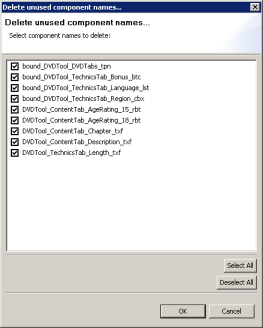
\includegraphics[width=0.60\textwidth]{52/ps/DeleteUnusedCompNames}
\caption{Deleting unused Component Names}
\label{RNDeleteUnusedCN}
\end{center}
\end{figure}
		
\end{itemize}

\textbf{HTML Test Result Reports can be expanded again}
\begin{itemize}
\item Following changes made for the initial contribution to Eclipse, the HTML Test Result Reports could not be viewed properly in the previous version. 
\item In this release, the nodes in the HTML reports can be expanded and collapsed to view the whole test progress. 

\begin{figure}[h]
\begin{center}
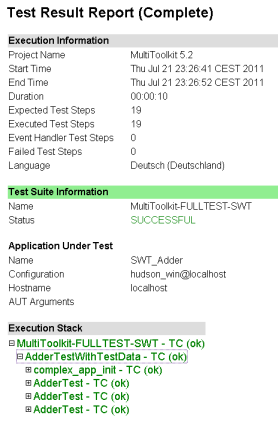
\includegraphics[width=0.60\textwidth]{52/ps/HTMLReport}
\caption{HTML Reports}
\label{RNHTMLReport}
\end{center}
\end{figure}
		
\end{itemize}

\textbf{State of component recognition displayed when collecting technical names}
\label{RNCompRec}
\begin{itemize}
\item When a component (technical name) is collected from an \gdaut{}, it receives a colored
dot corresponding to the accuracy of the object recognition for this component \textit{at the time of collecting}.
\begin{description}
\item [A green dot]{signifies that the component could be found with an exact match, and was the only component above the threshold}.
\item [A yellow dot]{means that the component is an exact match, but that multiple other components were also above the threshold.}
\item [A red dot]{ means that this component cannot be relocated in the current state of the \gdaut{}}
\end{description}
\item As a side effect, the colors on the component names (green) and technical names (red) that were displayed in previous versions are now no longer shown. Once the \gdomeditor{} has been saved, all names are shown with plain black icons. 
\begin{figure}[h]
\begin{center}
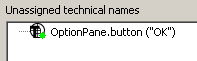
\includegraphics[width=0.6\textwidth]{52/ps/ColorDot}
\caption{Colored Dots for Object Mapping}
\label{RNColorDot}
\end{center}
\end{figure}
\end{itemize}

\textbf{Migration wizard re-enabled}
\begin{itemize}
\item  When migrating to the new version of \app{}, the migration assistant will automatically notify you that your database scheme is out-of-date. 
\item You can then select which \gdprojects{} to import (these must have been exported from the \gddb{} prior to migrating!).
\item The assistant will drop the tables in the \gddb{}, recreate the necessary tables and import the \gdprojects{} you specified.

\begin{figure}[h]
\begin{center}
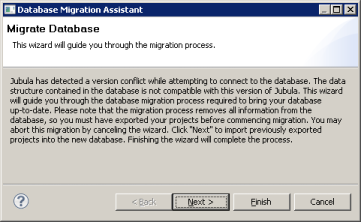
\includegraphics[width=0.6\textwidth]{52/ps/Migration}
\caption{Migration Wizard}
\label{RNMigration}
\end{center}
\end{figure}

\end{itemize}


\textbf{Copy ID to Clipboard also for \gdsuites{}}
\begin{itemize}
\item The ability to copy a unique ID to the clipboard to reference a \app{} element in external systems has also been implemented for \gdsuites{}. 
\item You can now copy the ID of a \gdcase{} or a \gdsuite{} to the clipboard, and also open an element based on its ID in the clipboard using \bxkey{Shift+F9}
\end{itemize}

\textbf{The DBTool is more verbose}
\begin{itemize}
\item The command line tool to import, export and delete \gdprojects{} in the \gddb{}, the DBTool, has been updated so that it is more verbose.
\end{itemize}

\textbf{Progress View}
\begin{itemize}
\item The \ite{} now  uses the progress view to show longer-running activities such as test execution, connecting to \gdauts{} etc.
\end{itemize}

\textbf{Edit Parameters Dialog in \gddataeditor{} can be opened via double-click}
\begin{itemize}
\item In the \gddataeditor{}  it is no longer necessary to open the Edit Parameters Dialog via context-menu, as it can now also be opened via double-click on the data set you wish to edit.
\end{itemize}


\textbf{Mac keyboards now supported, new mechanism for adding keyboard layout files}
\begin{itemize}
\item In the \gdaut{} configuration dialog for SWT and RCP \gdauts{}, the \bxname{Keyboard Layout} combo box now only offers 
layouts that have been defined for \app{}. German (DE) and English (US) are defined as standard. 
\item As well as being able to add keyboard layouts for other keyboards, you can also define platform-specific keyboard layouts (e.g. for Mac)
\item The documentation has been updated to describe the new mechanism for adding keyboard layouts.
\end{itemize}

\textbf{Object mapping: Degree of recognition accuracy for a test run can be viewed}
\begin{itemize}
\item The \gdomeditor{} has been extended so that the accuracy of component recognition is persisted and can be displayed.  
\item As well as displaying the state of component recognition when a technical name is collected from the \gdaut{} \bxpref{RNCompRec}, the degree of recognition accuracy is also noted 
for each test run. 
\item You can see the values for the recognition accuracy in two new BIRT reports in \app{}.
\begin{description}
\item [OMNameQuality]{shows a breakdown of the component names used in your test, and displays the degree of accuracy they were located during the test. You can use this report to see whether there are any component names that may need to be remapped (i.e. who are close to the threshold of not being found) before the test encounters a \bxname{Component Not Found} error. }
\item [OMNameQualityChart]{This report is a visual (graph) representation of the accuracy with which components were located during the test run. You can use the report to help you decide which components may need to be remapped, as they may soon result in a \bxname{Component Not Found} error during the test.}
\end{description}
\end{itemize}

\textbf{Mylyn: Refactored \gdcases{} are added to context}
\begin{itemize}
\item When working on a Mylyn task in app{}, \gdcases{} you create using the \bxname{refactor} function are now automatically added to the context.
\end{itemize}

\textbf{Mylyn: \gdcases{} opened via \bxkey{Ctrl+Shift+T} are added to context}
\begin{itemize}
\item When working on a Mylyn task in \app{}, \gdcases{} opened using the key combination \bxkey{Ctrl+Shift+T} are now automatically added to the context.
\end{itemize}

\textbf{Mylyn: \gdcases{} added via \gdcase{} reference dialog are added to context}
\begin{itemize}
\item When working on a Mylyn task in \app{}, \gdcases{} added using the \bxname{Add \gdcase{} reference} dialog are now automatically added to the context.
\end{itemize}

\textbf{Teststyle: Rules can now be viewed via the \gdpropview{}}
\begin{itemize}
\item When working with Teststyle, you can now open the \gdproject{} properties dialog to see the rule that has been flouted via:\\
\bxmenu{Show Teststyle Rule}{}{}\\
from the \gdprobview{}.
\end{itemize}

\textbf{Changes to BIRT reports}
\begin{itemize}
\item The BIRT report GUIdancerFULL has been removed.
\item There are new BIRT reports:
\begin{itemize}
\item \bxname{GUIdancerComments} shows a table of all failed relevant tests for the time specified, including the comment title that can be entered in the \gdtestsummaryview{}. This report is useful for delivering daily status reports of the tests.
\item \bxname{GUIdancerDuration} shows the duration of the chosen tests.
\item \bxname{GUIdancerExecutionHistogram} shows the proportion of executed, failed and non-executed \gdsteps{} for a test. This report is most useful when one specific \gdsuite{} is compared to see its progress over time. 
\item \bxname{TestresultSummary} shows a table of the \gdtestsummaryview{} for the dates and tests chosen. 
\end{itemize}
\item You can now also enter the \gdjob{} as a parameter for the report. The \gdsuites{} in the \gdjob{} are still displayed individually, however. 
\end{itemize}



\textbf{License Dialog: Restart prompt}
\begin{itemize}
\item Once a license has been added via the Preferences, a dialog is shown to remind you to restart \app{} before continuing. 
\item From the dialog you can choose to restart \app{} automatically.
\end{itemize}


\subsection{Known issues and other information}

\textbf{Problem displaying component names from browsers}
\begin{itemize}
\item In some siutations, when viewing the \gdcompnamesview{} from a browser, you may see GUIDs (a long number/character string) instead of the component name.
\item This is a problem displaying the component name at the moment and can be considered a display error, albeit a serious one. 
\item The component names themselves are correct, and can be seen either by opening the editor, or by refreshing the \gdproject{}.
\end{itemize}

\textbf{Issue with incorrect handling of \bxshell{null} in renderers fixed}
\begin{itemize}
\item Renderers in Swing that return \bxshell{null} can now be correctly handled.
\item See \url{http://eclip.se/426978} for more details. 
\end{itemize}

\textbf{Selenium update}
\begin{itemize}
\item We have updated the version of Selenium used for HTML tests to 2.39.
\end{itemize}

\textbf{Port number for embedded \gdagent{} changed}
\begin{itemize}
\item The default port number for the embedded \gdagent{} is now 60001.
\item You can change the default port number in the preferences.
\end{itemize}

\textbf{Table view has been removed from the \gdomeditor{}}
\begin{itemize}
\item The table view has been removed from the \gdomeditor{}.
\end{itemize}

\textbf{Problems opening BIRT reports when using IE11}
\begin{itemize}
\item There is a known issue with BIRT reporting that occurs when using Internet Explorer 11. 
\item There is a ticket open in the \gd{} Bugzilla (\url{https://bugzilla.bredex.de/show_bug.cgi?id=1281}) and in the Eclipse Bugzilla (\url{http://eclip.se/422056}) for this. The ticket in the Eclipse Bugzilla documents workarounds.
\end{itemize}

\textbf{Java 1.4 \gdauts{} no longer testable}
\begin{itemize}
\item As of this version, Java 1.4 \gdauts{} are no longer testable with the \ite{}. 
\end{itemize}

\textbf{Changes to the launcher for the \gdagent{}}
\begin{itemize}
\item The \gdagent{} is no longer available under the name \bxshell{autagent-lin} or \bxshell{autagent-sol}.
\item Use the launcher \bxshell{autagent} instead.
\end{itemize}

\textbf{Java 7 tests on Mac}
\begin{itemize}
\item There are still some issues running tests on Mac machines with Java 7. We suggest using Java 6 on Mac machines for the moment.
\end{itemize}

\textbf{Working directory for \ite{} and \gdagent{} on Linux}
\begin{itemize}
\item The \gdagent{} and the \ite{} now  use the current directory as their working directory on Linux systems.
\end{itemize}


\textbf{The \ite{} now uses Java 7}
\begin{itemize}
\item We have updated the version of Java installed with the \ite{} to version 7.
\end{itemize}

\textbf{The installer requires Java 7}
\begin{itemize}
\item You will need Java 7 installed to be able to run the installer.
\end{itemize}

\textbf{iOS 5.0 no longer supported}
\begin{itemize}
\item We no longer support testing on iOS 5.0 \gdauts{}.
\end{itemize}

\textbf{Working with RDP connections on Windows 8}
\begin{itemize}
\item Windows 8 users working with RDP connections for test execution should ensure that they have installed all updates for Windows. 
\end{itemize}

\textbf{Updated the version of EclipseLink used}
\begin{itemize}
\item In this version, we have switched to EclipseLink 2.5.1 and JPA 2.1.0.
\end{itemize}

\textbf{Vista support removed}
\begin{itemize}
\item We no longer execute tests on Vista: the support for Vista has been removed for this version.
\end{itemize}

\textbf{Multi-window mode for HTML testing on Mac OSX}
\begin{itemize}
\item There are known issues with starting \gdauts{} that are using the multi-window mode on Mac OSX, both in Firefox and Safari.
\item We have removed these combinations from our tests.
\end{itemize}

\textbf{Pure SWT \gdauts{} no longer tested}
\begin{itemize}
\item We no longer execute regression tests on pure SWT \gdauts{}. We do, however, perform various tests on RCP, which uses SWT components. 
\end{itemize}

\textbf{\gdagent{} started without console per default}
\begin{itemize}
\item The standalone \gdagent{} is now started without a console per default.
\item If you would like to see the console when starting the \gdagent{}, you must adapt the \bxname{autagent.ini} file.
\item In the -vm parameter, use \bxname{java} instead of \bxname{javaw}.
\end{itemize}


\section{Release Notes for \app{} version 6.0007x}

\subsection{New Features and Developments}

\textbf{Embedded gdagent{}}\\
\begin{itemize}
\item If you are starting your \gdaut{} and running your tests on your local machine, 
you can now connect to an embedded \gdagent{} directly from the \ite. 
\item This saves you having to start an \gdagent{} on localhost. 
\item This is also useful for testers working with \jb{} as a feature in an Eclipse installation. 
\item The embedded \gdagent{} is started on port 60000 by default; this number can be changed in the preferences.

\begin{figure}[h]
\begin{center}
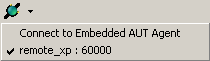
\includegraphics[width=0.60\textwidth]{52/ps/EmbeddedAgent}
\caption{Embedded AUT Agent}
\label{RNEmbeddedAgent}
\end{center}
\end{figure}


\end{itemize}


\textbf{Refactor: Replace with \gdcase{}}
\begin{itemize}
\item In the \gdtestcaseeditor{} and \gdtestsuiteeditor{}, there is a new option to replace one or more selected \gdcases{} with another \gdcase{} from the library. 
\item A new wizard takes you step-by-step through the replacement process, letting you transfer component names, match parameters and add further information for the new \gdcase{}.
\item This feature should help testers who want to restructure their tests after creating a reusable module to replace one or more \gdcases{}. 
\end{itemize}

\textbf{\gdomeditor{}: Cleanup unused component names}

\begin{itemize}
\item In the \gdomeditor{}, there is a new option in the context-sensitive menu. 
\item Via \bxmenu{Cleanup}{unused component names}{} \\
you can start a search for any component names that are no longer used in \gdsuites{} for this \gdaut{}. 
\item Once the search is finished, you can delete all of these unused names from the \gdomeditor{}. If they are then no longer used in the entire \gdproject{}, 
they can be deleted from the \gdcompnamebrowser{}. 

\begin{figure}[h]
\begin{center}
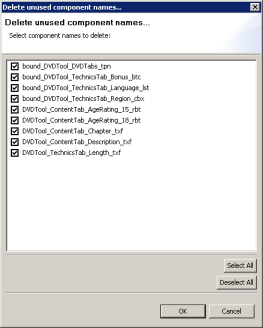
\includegraphics[width=0.60\textwidth]{52/ps/DeleteUnusedCompNames}
\caption{Deleting unused Component Names}
\label{RNDeleteUnusedCN}
\end{center}
\end{figure}
		
\end{itemize}

\textbf{HTML Test Result Reports can be expanded again}
\begin{itemize}
\item Following changes made for the initial contribution to Eclipse, the HTML Test Result Reports could not be viewed properly in the previous version. 
\item In this release, the nodes in the HTML reports can be expanded and collapsed to view the whole test progress. 

\begin{figure}[h]
\begin{center}
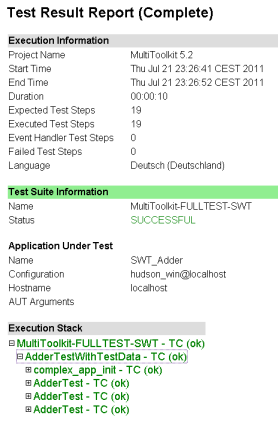
\includegraphics[width=0.60\textwidth]{52/ps/HTMLReport}
\caption{HTML Reports}
\label{RNHTMLReport}
\end{center}
\end{figure}
		
\end{itemize}

\textbf{State of component recognition displayed when collecting technical names}
\label{RNCompRec}
\begin{itemize}
\item When a component (technical name) is collected from an \gdaut{}, it receives a colored
dot corresponding to the accuracy of the object recognition for this component \textit{at the time of collecting}.
\begin{description}
\item [A green dot]{signifies that the component could be found with an exact match, and was the only component above the threshold}.
\item [A yellow dot]{means that the component is an exact match, but that multiple other components were also above the threshold.}
\item [A red dot]{ means that this component cannot be relocated in the current state of the \gdaut{}}
\end{description}
\item As a side effect, the colors on the component names (green) and technical names (red) that were displayed in previous versions are now no longer shown. Once the \gdomeditor{} has been saved, all names are shown with plain black icons. 
\begin{figure}[h]
\begin{center}
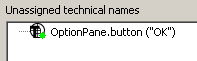
\includegraphics[width=0.6\textwidth]{52/ps/ColorDot}
\caption{Colored Dots for Object Mapping}
\label{RNColorDot}
\end{center}
\end{figure}
\end{itemize}

\textbf{Migration wizard re-enabled}
\begin{itemize}
\item  When migrating to the new version of \app{}, the migration assistant will automatically notify you that your database scheme is out-of-date. 
\item You can then select which \gdprojects{} to import (these must have been exported from the \gddb{} prior to migrating!).
\item The assistant will drop the tables in the \gddb{}, recreate the necessary tables and import the \gdprojects{} you specified.

\begin{figure}[h]
\begin{center}
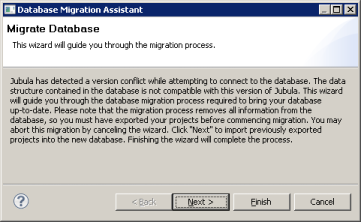
\includegraphics[width=0.6\textwidth]{52/ps/Migration}
\caption{Migration Wizard}
\label{RNMigration}
\end{center}
\end{figure}

\end{itemize}


\textbf{Copy ID to Clipboard also for \gdsuites{}}
\begin{itemize}
\item The ability to copy a unique ID to the clipboard to reference a \app{} element in external systems has also been implemented for \gdsuites{}. 
\item You can now copy the ID of a \gdcase{} or a \gdsuite{} to the clipboard, and also open an element based on its ID in the clipboard using \bxkey{Shift+F9}
\end{itemize}

\textbf{The DBTool is more verbose}
\begin{itemize}
\item The command line tool to import, export and delete \gdprojects{} in the \gddb{}, the DBTool, has been updated so that it is more verbose.
\end{itemize}

\textbf{Progress View}
\begin{itemize}
\item The \ite{} now  uses the progress view to show longer-running activities such as test execution, connecting to \gdauts{} etc.
\end{itemize}

\textbf{Edit Parameters Dialog in \gddataeditor{} can be opened via double-click}
\begin{itemize}
\item In the \gddataeditor{}  it is no longer necessary to open the Edit Parameters Dialog via context-menu, as it can now also be opened via double-click on the data set you wish to edit.
\end{itemize}


\textbf{Mac keyboards now supported, new mechanism for adding keyboard layout files}
\begin{itemize}
\item In the \gdaut{} configuration dialog for SWT and RCP \gdauts{}, the \bxname{Keyboard Layout} combo box now only offers 
layouts that have been defined for \app{}. German (DE) and English (US) are defined as standard. 
\item As well as being able to add keyboard layouts for other keyboards, you can also define platform-specific keyboard layouts (e.g. for Mac)
\item The documentation has been updated to describe the new mechanism for adding keyboard layouts.
\end{itemize}

\textbf{Object mapping: Degree of recognition accuracy for a test run can be viewed}
\begin{itemize}
\item The \gdomeditor{} has been extended so that the accuracy of component recognition is persisted and can be displayed.  
\item As well as displaying the state of component recognition when a technical name is collected from the \gdaut{} \bxpref{RNCompRec}, the degree of recognition accuracy is also noted 
for each test run. 
\item You can see the values for the recognition accuracy in two new BIRT reports in \app{}.
\begin{description}
\item [OMNameQuality]{shows a breakdown of the component names used in your test, and displays the degree of accuracy they were located during the test. You can use this report to see whether there are any component names that may need to be remapped (i.e. who are close to the threshold of not being found) before the test encounters a \bxname{Component Not Found} error. }
\item [OMNameQualityChart]{This report is a visual (graph) representation of the accuracy with which components were located during the test run. You can use the report to help you decide which components may need to be remapped, as they may soon result in a \bxname{Component Not Found} error during the test.}
\end{description}
\end{itemize}

\textbf{Mylyn: Refactored \gdcases{} are added to context}
\begin{itemize}
\item When working on a Mylyn task in app{}, \gdcases{} you create using the \bxname{refactor} function are now automatically added to the context.
\end{itemize}

\textbf{Mylyn: \gdcases{} opened via \bxkey{Ctrl+Shift+T} are added to context}
\begin{itemize}
\item When working on a Mylyn task in \app{}, \gdcases{} opened using the key combination \bxkey{Ctrl+Shift+T} are now automatically added to the context.
\end{itemize}

\textbf{Mylyn: \gdcases{} added via \gdcase{} reference dialog are added to context}
\begin{itemize}
\item When working on a Mylyn task in \app{}, \gdcases{} added using the \bxname{Add \gdcase{} reference} dialog are now automatically added to the context.
\end{itemize}

\textbf{Teststyle: Rules can now be viewed via the \gdpropview{}}
\begin{itemize}
\item When working with Teststyle, you can now open the \gdproject{} properties dialog to see the rule that has been flouted via:\\
\bxmenu{Show Teststyle Rule}{}{}\\
from the \gdprobview{}.
\end{itemize}

\textbf{Changes to BIRT reports}
\begin{itemize}
\item The BIRT report GUIdancerFULL has been removed.
\item There are new BIRT reports:
\begin{itemize}
\item \bxname{GUIdancerComments} shows a table of all failed relevant tests for the time specified, including the comment title that can be entered in the \gdtestsummaryview{}. This report is useful for delivering daily status reports of the tests.
\item \bxname{GUIdancerDuration} shows the duration of the chosen tests.
\item \bxname{GUIdancerExecutionHistogram} shows the proportion of executed, failed and non-executed \gdsteps{} for a test. This report is most useful when one specific \gdsuite{} is compared to see its progress over time. 
\item \bxname{TestresultSummary} shows a table of the \gdtestsummaryview{} for the dates and tests chosen. 
\end{itemize}
\item You can now also enter the \gdjob{} as a parameter for the report. The \gdsuites{} in the \gdjob{} are still displayed individually, however. 
\end{itemize}



\textbf{License Dialog: Restart prompt}
\begin{itemize}
\item Once a license has been added via the Preferences, a dialog is shown to remind you to restart \app{} before continuing. 
\item From the dialog you can choose to restart \app{} automatically.
\end{itemize}


\subsection{Known issues and other information}

\textbf{Problem displaying component names from browsers}
\begin{itemize}
\item In some siutations, when viewing the \gdcompnamesview{} from a browser, you may see GUIDs (a long number/character string) instead of the component name.
\item This is a problem displaying the component name at the moment and can be considered a display error, albeit a serious one. 
\item The component names themselves are correct, and can be seen either by opening the editor, or by refreshing the \gdproject{}.
\end{itemize}

\textbf{Issue with incorrect handling of \bxshell{null} in renderers fixed}
\begin{itemize}
\item Renderers in Swing that return \bxshell{null} can now be correctly handled.
\item See \url{http://eclip.se/426978} for more details. 
\end{itemize}

\textbf{Selenium update}
\begin{itemize}
\item We have updated the version of Selenium used for HTML tests to 2.39.
\end{itemize}

\textbf{Port number for embedded \gdagent{} changed}
\begin{itemize}
\item The default port number for the embedded \gdagent{} is now 60001.
\item You can change the default port number in the preferences.
\end{itemize}

\textbf{Table view has been removed from the \gdomeditor{}}
\begin{itemize}
\item The table view has been removed from the \gdomeditor{}.
\end{itemize}

\textbf{Problems opening BIRT reports when using IE11}
\begin{itemize}
\item There is a known issue with BIRT reporting that occurs when using Internet Explorer 11. 
\item There is a ticket open in the \gd{} Bugzilla (\url{https://bugzilla.bredex.de/show_bug.cgi?id=1281}) and in the Eclipse Bugzilla (\url{http://eclip.se/422056}) for this. The ticket in the Eclipse Bugzilla documents workarounds.
\end{itemize}

\textbf{Java 1.4 \gdauts{} no longer testable}
\begin{itemize}
\item As of this version, Java 1.4 \gdauts{} are no longer testable with the \ite{}. 
\end{itemize}

\textbf{Changes to the launcher for the \gdagent{}}
\begin{itemize}
\item The \gdagent{} is no longer available under the name \bxshell{autagent-lin} or \bxshell{autagent-sol}.
\item Use the launcher \bxshell{autagent} instead.
\end{itemize}

\textbf{Java 7 tests on Mac}
\begin{itemize}
\item There are still some issues running tests on Mac machines with Java 7. We suggest using Java 6 on Mac machines for the moment.
\end{itemize}

\textbf{Working directory for \ite{} and \gdagent{} on Linux}
\begin{itemize}
\item The \gdagent{} and the \ite{} now  use the current directory as their working directory on Linux systems.
\end{itemize}


\textbf{The \ite{} now uses Java 7}
\begin{itemize}
\item We have updated the version of Java installed with the \ite{} to version 7.
\end{itemize}

\textbf{The installer requires Java 7}
\begin{itemize}
\item You will need Java 7 installed to be able to run the installer.
\end{itemize}

\textbf{iOS 5.0 no longer supported}
\begin{itemize}
\item We no longer support testing on iOS 5.0 \gdauts{}.
\end{itemize}

\textbf{Working with RDP connections on Windows 8}
\begin{itemize}
\item Windows 8 users working with RDP connections for test execution should ensure that they have installed all updates for Windows. 
\end{itemize}

\textbf{Updated the version of EclipseLink used}
\begin{itemize}
\item In this version, we have switched to EclipseLink 2.5.1 and JPA 2.1.0.
\end{itemize}

\textbf{Vista support removed}
\begin{itemize}
\item We no longer execute tests on Vista: the support for Vista has been removed for this version.
\end{itemize}

\textbf{Multi-window mode for HTML testing on Mac OSX}
\begin{itemize}
\item There are known issues with starting \gdauts{} that are using the multi-window mode on Mac OSX, both in Firefox and Safari.
\item We have removed these combinations from our tests.
\end{itemize}

\textbf{Pure SWT \gdauts{} no longer tested}
\begin{itemize}
\item We no longer execute regression tests on pure SWT \gdauts{}. We do, however, perform various tests on RCP, which uses SWT components. 
\end{itemize}

\textbf{\gdagent{} started without console per default}
\begin{itemize}
\item The standalone \gdagent{} is now started without a console per default.
\item If you would like to see the console when starting the \gdagent{}, you must adapt the \bxname{autagent.ini} file.
\item In the -vm parameter, use \bxname{java} instead of \bxname{javaw}.
\end{itemize}


\section{Release Notes for \app{} version 6.0007x}

\subsection{New Features and Developments}

\textbf{Embedded gdagent{}}\\
\begin{itemize}
\item If you are starting your \gdaut{} and running your tests on your local machine, 
you can now connect to an embedded \gdagent{} directly from the \ite. 
\item This saves you having to start an \gdagent{} on localhost. 
\item This is also useful for testers working with \jb{} as a feature in an Eclipse installation. 
\item The embedded \gdagent{} is started on port 60000 by default; this number can be changed in the preferences.

\begin{figure}[h]
\begin{center}
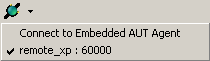
\includegraphics[width=0.60\textwidth]{52/ps/EmbeddedAgent}
\caption{Embedded AUT Agent}
\label{RNEmbeddedAgent}
\end{center}
\end{figure}


\end{itemize}


\textbf{Refactor: Replace with \gdcase{}}
\begin{itemize}
\item In the \gdtestcaseeditor{} and \gdtestsuiteeditor{}, there is a new option to replace one or more selected \gdcases{} with another \gdcase{} from the library. 
\item A new wizard takes you step-by-step through the replacement process, letting you transfer component names, match parameters and add further information for the new \gdcase{}.
\item This feature should help testers who want to restructure their tests after creating a reusable module to replace one or more \gdcases{}. 
\end{itemize}

\textbf{\gdomeditor{}: Cleanup unused component names}

\begin{itemize}
\item In the \gdomeditor{}, there is a new option in the context-sensitive menu. 
\item Via \bxmenu{Cleanup}{unused component names}{} \\
you can start a search for any component names that are no longer used in \gdsuites{} for this \gdaut{}. 
\item Once the search is finished, you can delete all of these unused names from the \gdomeditor{}. If they are then no longer used in the entire \gdproject{}, 
they can be deleted from the \gdcompnamebrowser{}. 

\begin{figure}[h]
\begin{center}
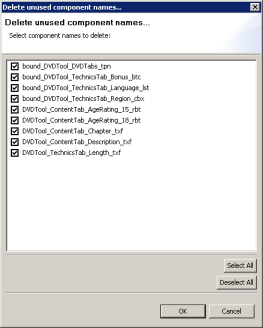
\includegraphics[width=0.60\textwidth]{52/ps/DeleteUnusedCompNames}
\caption{Deleting unused Component Names}
\label{RNDeleteUnusedCN}
\end{center}
\end{figure}
		
\end{itemize}

\textbf{HTML Test Result Reports can be expanded again}
\begin{itemize}
\item Following changes made for the initial contribution to Eclipse, the HTML Test Result Reports could not be viewed properly in the previous version. 
\item In this release, the nodes in the HTML reports can be expanded and collapsed to view the whole test progress. 

\begin{figure}[h]
\begin{center}
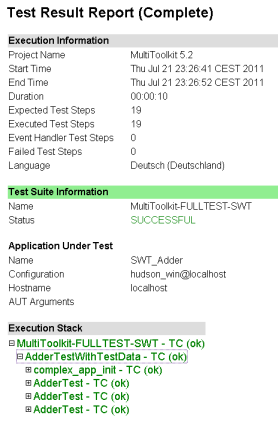
\includegraphics[width=0.60\textwidth]{52/ps/HTMLReport}
\caption{HTML Reports}
\label{RNHTMLReport}
\end{center}
\end{figure}
		
\end{itemize}

\textbf{State of component recognition displayed when collecting technical names}
\label{RNCompRec}
\begin{itemize}
\item When a component (technical name) is collected from an \gdaut{}, it receives a colored
dot corresponding to the accuracy of the object recognition for this component \textit{at the time of collecting}.
\begin{description}
\item [A green dot]{signifies that the component could be found with an exact match, and was the only component above the threshold}.
\item [A yellow dot]{means that the component is an exact match, but that multiple other components were also above the threshold.}
\item [A red dot]{ means that this component cannot be relocated in the current state of the \gdaut{}}
\end{description}
\item As a side effect, the colors on the component names (green) and technical names (red) that were displayed in previous versions are now no longer shown. Once the \gdomeditor{} has been saved, all names are shown with plain black icons. 
\begin{figure}[h]
\begin{center}
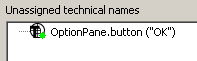
\includegraphics[width=0.6\textwidth]{52/ps/ColorDot}
\caption{Colored Dots for Object Mapping}
\label{RNColorDot}
\end{center}
\end{figure}
\end{itemize}

\textbf{Migration wizard re-enabled}
\begin{itemize}
\item  When migrating to the new version of \app{}, the migration assistant will automatically notify you that your database scheme is out-of-date. 
\item You can then select which \gdprojects{} to import (these must have been exported from the \gddb{} prior to migrating!).
\item The assistant will drop the tables in the \gddb{}, recreate the necessary tables and import the \gdprojects{} you specified.

\begin{figure}[h]
\begin{center}
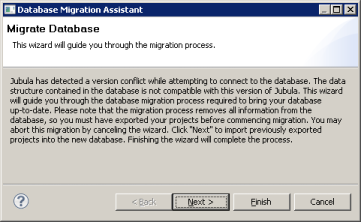
\includegraphics[width=0.6\textwidth]{52/ps/Migration}
\caption{Migration Wizard}
\label{RNMigration}
\end{center}
\end{figure}

\end{itemize}


\textbf{Copy ID to Clipboard also for \gdsuites{}}
\begin{itemize}
\item The ability to copy a unique ID to the clipboard to reference a \app{} element in external systems has also been implemented for \gdsuites{}. 
\item You can now copy the ID of a \gdcase{} or a \gdsuite{} to the clipboard, and also open an element based on its ID in the clipboard using \bxkey{Shift+F9}
\end{itemize}

\textbf{The DBTool is more verbose}
\begin{itemize}
\item The command line tool to import, export and delete \gdprojects{} in the \gddb{}, the DBTool, has been updated so that it is more verbose.
\end{itemize}

\textbf{Progress View}
\begin{itemize}
\item The \ite{} now  uses the progress view to show longer-running activities such as test execution, connecting to \gdauts{} etc.
\end{itemize}

\textbf{Edit Parameters Dialog in \gddataeditor{} can be opened via double-click}
\begin{itemize}
\item In the \gddataeditor{}  it is no longer necessary to open the Edit Parameters Dialog via context-menu, as it can now also be opened via double-click on the data set you wish to edit.
\end{itemize}


\textbf{Mac keyboards now supported, new mechanism for adding keyboard layout files}
\begin{itemize}
\item In the \gdaut{} configuration dialog for SWT and RCP \gdauts{}, the \bxname{Keyboard Layout} combo box now only offers 
layouts that have been defined for \app{}. German (DE) and English (US) are defined as standard. 
\item As well as being able to add keyboard layouts for other keyboards, you can also define platform-specific keyboard layouts (e.g. for Mac)
\item The documentation has been updated to describe the new mechanism for adding keyboard layouts.
\end{itemize}

\textbf{Object mapping: Degree of recognition accuracy for a test run can be viewed}
\begin{itemize}
\item The \gdomeditor{} has been extended so that the accuracy of component recognition is persisted and can be displayed.  
\item As well as displaying the state of component recognition when a technical name is collected from the \gdaut{} \bxpref{RNCompRec}, the degree of recognition accuracy is also noted 
for each test run. 
\item You can see the values for the recognition accuracy in two new BIRT reports in \app{}.
\begin{description}
\item [OMNameQuality]{shows a breakdown of the component names used in your test, and displays the degree of accuracy they were located during the test. You can use this report to see whether there are any component names that may need to be remapped (i.e. who are close to the threshold of not being found) before the test encounters a \bxname{Component Not Found} error. }
\item [OMNameQualityChart]{This report is a visual (graph) representation of the accuracy with which components were located during the test run. You can use the report to help you decide which components may need to be remapped, as they may soon result in a \bxname{Component Not Found} error during the test.}
\end{description}
\end{itemize}

\textbf{Mylyn: Refactored \gdcases{} are added to context}
\begin{itemize}
\item When working on a Mylyn task in app{}, \gdcases{} you create using the \bxname{refactor} function are now automatically added to the context.
\end{itemize}

\textbf{Mylyn: \gdcases{} opened via \bxkey{Ctrl+Shift+T} are added to context}
\begin{itemize}
\item When working on a Mylyn task in \app{}, \gdcases{} opened using the key combination \bxkey{Ctrl+Shift+T} are now automatically added to the context.
\end{itemize}

\textbf{Mylyn: \gdcases{} added via \gdcase{} reference dialog are added to context}
\begin{itemize}
\item When working on a Mylyn task in \app{}, \gdcases{} added using the \bxname{Add \gdcase{} reference} dialog are now automatically added to the context.
\end{itemize}

\textbf{Teststyle: Rules can now be viewed via the \gdpropview{}}
\begin{itemize}
\item When working with Teststyle, you can now open the \gdproject{} properties dialog to see the rule that has been flouted via:\\
\bxmenu{Show Teststyle Rule}{}{}\\
from the \gdprobview{}.
\end{itemize}

\textbf{Changes to BIRT reports}
\begin{itemize}
\item The BIRT report GUIdancerFULL has been removed.
\item There are new BIRT reports:
\begin{itemize}
\item \bxname{GUIdancerComments} shows a table of all failed relevant tests for the time specified, including the comment title that can be entered in the \gdtestsummaryview{}. This report is useful for delivering daily status reports of the tests.
\item \bxname{GUIdancerDuration} shows the duration of the chosen tests.
\item \bxname{GUIdancerExecutionHistogram} shows the proportion of executed, failed and non-executed \gdsteps{} for a test. This report is most useful when one specific \gdsuite{} is compared to see its progress over time. 
\item \bxname{TestresultSummary} shows a table of the \gdtestsummaryview{} for the dates and tests chosen. 
\end{itemize}
\item You can now also enter the \gdjob{} as a parameter for the report. The \gdsuites{} in the \gdjob{} are still displayed individually, however. 
\end{itemize}



\textbf{License Dialog: Restart prompt}
\begin{itemize}
\item Once a license has been added via the Preferences, a dialog is shown to remind you to restart \app{} before continuing. 
\item From the dialog you can choose to restart \app{} automatically.
\end{itemize}


\subsection{Known issues and other information}

\textbf{Problem displaying component names from browsers}
\begin{itemize}
\item In some siutations, when viewing the \gdcompnamesview{} from a browser, you may see GUIDs (a long number/character string) instead of the component name.
\item This is a problem displaying the component name at the moment and can be considered a display error, albeit a serious one. 
\item The component names themselves are correct, and can be seen either by opening the editor, or by refreshing the \gdproject{}.
\end{itemize}

\textbf{Issue with incorrect handling of \bxshell{null} in renderers fixed}
\begin{itemize}
\item Renderers in Swing that return \bxshell{null} can now be correctly handled.
\item See \url{http://eclip.se/426978} for more details. 
\end{itemize}

\textbf{Selenium update}
\begin{itemize}
\item We have updated the version of Selenium used for HTML tests to 2.39.
\end{itemize}

\textbf{Port number for embedded \gdagent{} changed}
\begin{itemize}
\item The default port number for the embedded \gdagent{} is now 60001.
\item You can change the default port number in the preferences.
\end{itemize}

\textbf{Table view has been removed from the \gdomeditor{}}
\begin{itemize}
\item The table view has been removed from the \gdomeditor{}.
\end{itemize}

\textbf{Problems opening BIRT reports when using IE11}
\begin{itemize}
\item There is a known issue with BIRT reporting that occurs when using Internet Explorer 11. 
\item There is a ticket open in the \gd{} Bugzilla (\url{https://bugzilla.bredex.de/show_bug.cgi?id=1281}) and in the Eclipse Bugzilla (\url{http://eclip.se/422056}) for this. The ticket in the Eclipse Bugzilla documents workarounds.
\end{itemize}

\textbf{Java 1.4 \gdauts{} no longer testable}
\begin{itemize}
\item As of this version, Java 1.4 \gdauts{} are no longer testable with the \ite{}. 
\end{itemize}

\textbf{Changes to the launcher for the \gdagent{}}
\begin{itemize}
\item The \gdagent{} is no longer available under the name \bxshell{autagent-lin} or \bxshell{autagent-sol}.
\item Use the launcher \bxshell{autagent} instead.
\end{itemize}

\textbf{Java 7 tests on Mac}
\begin{itemize}
\item There are still some issues running tests on Mac machines with Java 7. We suggest using Java 6 on Mac machines for the moment.
\end{itemize}

\textbf{Working directory for \ite{} and \gdagent{} on Linux}
\begin{itemize}
\item The \gdagent{} and the \ite{} now  use the current directory as their working directory on Linux systems.
\end{itemize}


\textbf{The \ite{} now uses Java 7}
\begin{itemize}
\item We have updated the version of Java installed with the \ite{} to version 7.
\end{itemize}

\textbf{The installer requires Java 7}
\begin{itemize}
\item You will need Java 7 installed to be able to run the installer.
\end{itemize}

\textbf{iOS 5.0 no longer supported}
\begin{itemize}
\item We no longer support testing on iOS 5.0 \gdauts{}.
\end{itemize}

\textbf{Working with RDP connections on Windows 8}
\begin{itemize}
\item Windows 8 users working with RDP connections for test execution should ensure that they have installed all updates for Windows. 
\end{itemize}

\textbf{Updated the version of EclipseLink used}
\begin{itemize}
\item In this version, we have switched to EclipseLink 2.5.1 and JPA 2.1.0.
\end{itemize}

\textbf{Vista support removed}
\begin{itemize}
\item We no longer execute tests on Vista: the support for Vista has been removed for this version.
\end{itemize}

\textbf{Multi-window mode for HTML testing on Mac OSX}
\begin{itemize}
\item There are known issues with starting \gdauts{} that are using the multi-window mode on Mac OSX, both in Firefox and Safari.
\item We have removed these combinations from our tests.
\end{itemize}

\textbf{Pure SWT \gdauts{} no longer tested}
\begin{itemize}
\item We no longer execute regression tests on pure SWT \gdauts{}. We do, however, perform various tests on RCP, which uses SWT components. 
\end{itemize}

\textbf{\gdagent{} started without console per default}
\begin{itemize}
\item The standalone \gdagent{} is now started without a console per default.
\item If you would like to see the console when starting the \gdagent{}, you must adapt the \bxname{autagent.ini} file.
\item In the -vm parameter, use \bxname{java} instead of \bxname{javaw}.
\end{itemize}


\makeatletter
\section{Release Notes for version 4.3.01105}
\makeatother
\subsection{Information}
This release is a patch to fix a problem that occurred in the \bxname{unbound modules concrete} whereby the \bxname{tree} component had a false component type. The database and license are the same as in version 4.3.01105. 

\makeatletter
\section{Release Notes for version 4.3.01105}
\makeatother
\subsection{New features and developments}
\textbf{Mylyn integration}
\begin{itemize}
\item The Mylyn plugin is now available for use within the \ite{}. 
\item You can connect to repositories (e.g. bug-tracking systems) to work on testing tasks directly in the \ite{}.
\item You can also create your own local tasks, and reduce the amount of \gdcases{} visible to only those required for the current task.
\end{itemize}
\textbf{Central test data}
\begin{itemize}
\item The \ite{} has a new editor for managing data centrally for a \gdproject{}
\item The \gddataeditor{} can be opened via a button on the toolbar.
\item Within the editor, you can add data sets which can then be referenced in \gdcases{}. 
\end{itemize}

\textbf{New data option and display in \gdpropview{}}
\begin{itemize}
\item The \gdpropview{} now shows what type of data is currently being used for a \gdcase{}.
\item The possible data sources are:
\begin{description}
\item [Referenced Test Case]{the data being used have come directly from the original specification of this \gdcase{}. }
\item [Local Test Case]{the data being used were entered for this \gdcase{}. You can change from \bxname{local} to \bxname{referenced} test data using the combo box to reset the default value from the referenced \gdcase{}.}
\item [Central test data set]{the data have come from a central test data set.}
\item [Excel data file]{an Excel file has been entered as the data source.}
\end{description}
\end{itemize}

\textbf{New search dialog and options}
\begin{itemize}
\item There are new options to search for items and test data within a \gdproject{}.
\item The search dialog can be opened from the toolbar and offers searches for:
\begin{description}
\item [Keywords]{Names of \gdsteps{}, \gdcases{}, \gdsuites{}, \gdjobs{} and categories in the \gdproject{}}
\item [Test data]{Data contained in \gdcases{}, \gdsteps{} and central data sets}
\item [Files]{File types and contents in the workspace}
\item [Tasks]{Tasks from repositories}
\end{description}
\item Search results are shown in the \gdsearchresultview{}. Items can be opened in their editors by double-clicking the specific search result. 
\end{itemize}

\textbf{Manual \gdsteps{}}
\begin{itemize}
\item You can now define manual \gdcases{}
\item There is a new module for a manual \gdstep{}.
\item Manual \gdcases{} can be combined into \gdsuites{} and executed.
\item During execution, a dialog appears to inform the manual tester which steps to perform.
\item The tester can mark the action as \bxname{passed} or \bxname{failed} and can write comments about the \gdstep{}.
\item The result reports from manual tests can be examined and analyzed just like result reports for automated tests.
\end{itemize}

\textbf{Testing \gdauts{} started by other \gdauts{}}
\begin{itemize}
\item It is now possible to test an \gdaut{} that was started by another \gdaut{}. 
\item There is a new mode for the \gdagent{} to allow this, the \bxname{lenient mode}.
\item \gdauts{} started in this way must be of the same toolkit as the original \gdaut{}.
\item For each newly started \gdaut{}, a new \gdaut{} ID is generated with a running number. 
\end{itemize}
\textbf{Test results}
\begin{itemize}
\item Test results that are reopened from the \gdtestsummaryview{} now contain complete information about each \gdstep{}.
\item Test results can also be exported from the \gdtestsummaryview{} in HTML and XML format.
\item The option to automatically clean up test result details is now part of the \gdproject{} properties, and no longer a user preference.
\item In the \gdtestsummaryview{}, you can now enter comments about each test run to document the reason for failing or passing. 
\end{itemize}
\textbf{New split pane view for the \gdomeditor{}}
\begin{itemize}
\item The \gdomeditor{} has a new view -- the split view.
\item In the split view, each category (\bxname{assigned names, unassigned component names} and \bxname{unassigned technical names}) has a different pane.
\item This allows you to navigate to the place you require in each category separately to make mapping in large \gdprojects{} more comfortable.
\end{itemize}
\textbf{New actions}
\begin{itemize}
\item Check existence of window by title
\item Check text at mouse position in trees
\item Store value at mouse position on trees
\item Store value on selected node in trees
\item Store value at mouse position in tables
\end{itemize}

\textbf{New parameters for existing actions}
\begin{itemize}
\item The action for selecting a node from a tree now also has the parameter \bxname{extend selection} so that multiple nodes can be selected in trees.
\item The parameters for actions requiring modifiers (control, alt etc.) have been changed so that a space-separated list of modifiers can be entered. Content assist is available for the modifier parameters.
\end{itemize}

\textbf{Protection for reused \gdprojects{}}
\begin{itemize}
\item There is a new option in the \gdproject{} wizard and \gdproject{} properties to \bxname{protect} a \gdproject{}. 
\item We recommend marking a \gdproject{} as protected if you are using it as a library (referenced) \gdproject{} for another \gdproject{}.
\item In protected \gdprojects{}, \gdcases{} cannot be deleted, and the \bxname{edit parameters} dialog cannot be opened. 
\item This is to stop any irrevocable changes being made that would affect the \gdprojects{} that reuse the protected \gdproject{}.
\item The protected status of \gdprojects{} can be altered in the \gdproject{} properties.
\end{itemize}
\textbf{Viewing BIRT reports in embedded database}
\begin{itemize}
\item BIRT reports generated from the \gdtestsummaryview{} can now be viewed when using the  embedded \gddb{}.
\end{itemize}
\textbf{Show where used on \gdsuite{}}
\begin{itemize}
\item The action \bxname{Show where used} (\bxkey{F6}) is now also possible on \gdsuites{} that have been reused in \gdjobs{}.
\end{itemize}
\textbf{Open specification action}
\begin{itemize}
\item There is a new action available on \gdcases{} and \gdsuites{} which have been reused (in other \gdcases{} or in \gdjobs{}). 
\item Use \bxkey{Ctrl+F6} to open the specification of the selected \gdcase{} or \gdsuite{} in the relevant editor.
\item This action is possible even if the \gdcase{} or \gdsuite{} to open is hidden due to an active filter. 
\end{itemize}
\textbf{Open \gdcase{} action}
\begin{itemize}
\item There is a new dialog to open an existing \gdcase{} or multiple \gdcases{} in their editors.
\item Use \bxkey{Ctrl+Shift+T} to open the dialog and select the \gdcases{} to be opened.
\item This action is possible even if the \gdcase{} or \gdsuite{} to open is hidden due to an active filter. 
\end{itemize}


\textbf{Show corresponding specification in \gdomeditor{}}
\begin{itemize}
\item In the \gdomeditor{} there is a new option to show the corresponding specification of a component name.
\item You can use this option when a component name appears in the \gdomeditor{} that you should have overwritten. 
\item The \gdsearchresultview{} only shows places which could have lead to this component name appearing in the \gdomeditor{}, not all places in the test where it has been used.
\end{itemize}

\textbf{Key combination to switch views in the client}
\begin{itemize}
\item We have introduced shortcuts to switch to specific views in the specification perspective.
\item To switch to the \gdtestsuitebrowser{}, use \bxkey{Alt+Shift+1}
\item To switch to the \gdtestcasebrowser{}, use \bxkey{Alt+Shift+2}
\item To switch to the \gdpropview{}, use \bxkey{Alt+1}
\item To switch to the \gddatasetsview{}, use \bxkey{Alt+2}
\item To switch to the \gdcompnamesview{}, use \bxkey{Alt+3}
\item To switch to editor, use \bxkey{F12}
\end{itemize}
The key combinations can be changed in the preferences. 

\textbf{Support for custom renderers in Swing}
\begin{itemize}
\item Custom renderers in Swing \gdauts{} can now be tested as long as the renderer implements either getText() or getTestableText(). 
\item The method signatures you implement must be:
\begin{quote}
public String getTestableText();
public String getText();
\end{quote}
\item If you don't have a getText() method, then we recommend using the getTestableText() option to avoid conflicts. 
\end{itemize}

\textbf{Dropping \gdcases{} directly into the editor area}
\begin{itemize}
\item You can now drop \gdcases{} directly into the editor, without having to place the \gdcase{} before or after another \gdcase{} in the editor.
\item The \gdcase{} is placed at the bottom of the tree in the editor.
\end{itemize}

\subsection{Other information}
\textbf{New workspace recommended for 4.3}
\begin{itemize}
\item We recommend setting up a new workspace for version 4.3. 
\end{itemize}
\textbf{Object mapping in RCP \gdauts{} that do not use GEF}
\begin{itemize}
\item We have fixed an issue with automatic component naming in RCP \gdauts{}.
\item Customers testing RCP \gdauts{} where \textbf{no} GEF bundles are present are advised to remap their components. 
\end{itemize}
\makeatletter
\section{Release Notes for version 4.2.01053}
\makeatother
\subsection{New features and developments}

\textbf{Eclipse 3.6 supported}
\begin{itemize}
\item Tests can be written for  Eclipse applications that are written in 3.6
\end{itemize}

\textbf{Viewing test results}
\begin{itemize}
\item Full test result details that are still in the \gddb{} can now be opened in the \gdtestresultview{} from the \gdtestsummaryview{}. 
\item This lets you review tests that ran overnight directly in the \ite{}. 
\end{itemize}

\textbf{Automatic \gddb{} migration}
\begin{itemize}
\item The \ite{} now contains a \gddb{} migration wizard.
\item When a connection to a \gddb{} is made in a new version, the \ite{} automatically recognizes whether the \gddb{} version is incompatile. 
\item If so, you can start the migration wizard. You specify which \gdprojects{} should be imported into the new \gddb{} (the \gdprojects must have been exported from the previous version).
\item The migration wizard converts the \gddb{} automatically to the new version.
\end{itemize}

\textbf{Commenting out \gdcases{}}
\begin{itemize}
\item You can now comment out \gdcases{} and \gdsteps{} in editors. 
\item Items that have been commented out are inactive and are neither validated for \gdsuite{} completeness, nor executed.
\end{itemize}

\textbf{New parameters for table actions}
\begin{itemize}
\item Actions on tables now have new parameters for \bxname{row operator} and \bxname{column operator}.
\item You can now select rows and columns based on their title and also determine how you want the selection to occur (equals, matches, simple match, not equals).
\end{itemize}

\textbf{New parameter for select actions}
\begin{itemize}
\item Actions that select items from tables, lists and trees have a new parameter for \bxname{mouse button}.
\item You can now define which mouse button should be used to select the item.
\end{itemize}

\textbf{Number of failed \gdsteps{} shown}
\begin{itemize}
\item The \gdtestsummaryview{} now also has the information about how many \gdsteps{} failed in a test run.
\end{itemize}

\textbf{Information about whether test result details are available}
\begin{itemize}
\item The \gdtestsummaryview{} now also has the information about whether the details for a test run are still in the \gddb{}.
\item If the results are still available, then the \gdtestresultview{} can be reopened.
\end{itemize}

\textbf{Spring to next/previous error}
\begin{itemize}
\item In the \gdtestresultview{} which opens when you open the results for a test run from the \gdtestsummaryview{}, you can use two new toolbar buttons to spring to the next/previous error.
\end{itemize}

\textbf{Showing comments for \gdcases{}}
\begin{itemize}
\item Any comments you write on \gdcases{} are now visible as a tooltip when you hover over the \gdcase{} in the browsers or in the search result view.
\end{itemize}

\textbf{Pause on error}
\begin{itemize}
\item There is a new button on the toolbar to pause the test execution if an error occurs.
\item This can be switched on and off during a test run and allows you to easily stop the test to see what went wrong.
\item The test can be continued by clicking the \bxname{pause test execution} button on the toolbar.
\end{itemize}

\textbf{Using running \gdaut{} details to define an \gdaut{}}
\begin{itemize}
\item \gdauts{} that have been started using the \bxname{gdrun} command can now be automatically defined in the \ite{}.
\item You can select the option to create an \gdaut{} definition from the running \gdauts{} view for any \gdaut{} that is currently unknown.
\end{itemize}

\textbf{Show referenced children}
\begin{itemize}
\item There is a new option in the preferences to show referenced children in \gdcases{} in the \gdtestcasebrowser{}.
\item This preference is activated by default. 
\item Deactivating the preference means that any children of referenced \gdcases{} are not displayed in the \gdtestcasebrowser{}. 
\item This can help in particularly large \gdprojects{} to inprove performance.
\end{itemize}


\textbf{New action}
\begin{itemize}
\item There is a new action to wait for the menu component.
\end{itemize}

\subsection{Other information}
\textbf{XML and HTML reports scheduled for removal}
\begin{itemize}
\item The XML and HTML reports that can be generated by the \ite{} (configurable in the preferences) are scheduled for removal in the next versions. 
\item There will be an alternative feature to create a HTML report from the test result report, as long as the test details are still in the \gddb{}.
\item For queries about this plan, please contact the support team.
\end{itemize}

\textbf{Deprecated unbound modules earlier than 3.0 scheduled for removal}
\begin{itemize}
\item The unbound modules that have been deprecated in versions earlier than 3.0 are also scheduled for removal in the upcoming version. 
\item We always recommend updating to the latest version of the unbound modules and removing any references to deprecated modules in your tests. 
\end{itemize}

\textbf{New unbound modules for tables and for select actions on lists, trees and tree-tables}
\begin{itemize}
\item Because we have added new parameters to actions on these components, there are new unbound modules for the actions.
\item The old unbound modules have been set to deprecated. 
\item We recommend updating any deprecated modules in your tests with the new modules.
\item You can see what the new module is by looking in the deprecated module - these now contain the new actions. 
\end{itemize}

\textbf{Merging in the \gdomeditor}
\begin{itemize}
\item The option to merge components in the \gdomeditor{} has been temporarily deactivated for this release. 
\end{itemize}

\makeatletter
\section{Release Notes for version 4.1.01039}
\makeatother
\subsection{New features and developments}
\textbf{New option in delete \gdproject{} dialog}
\begin{itemize}
\item When you delete a \gdproject{}, you can now decide whether you want to keep the test results for the \gdproject{} or delete them as well.
\end{itemize}
\textbf{Performance improvements}
\begin{itemize}
\item We have further improved the performance for the saving and loading of \gdprojects{}. The validation of \gdsuites{} now runs as a background job so that test specification can continue while the tests are being validated.
\item \gdsuites{} must be validated before they can be executed. 
\end{itemize}
\textbf{Generated names penalty removed}
\begin{itemize}
\item The generated names penalty has been removed from the object mapping configuration area and from the object recognition calculation.
\end{itemize}
\textbf{Optional automatic screenshots when errors occur}
\begin{itemize}
\item You can now define whether or not screenshots should automatically be taken when an error occurs. 
\item Screenshots taken in this manner are saved into the \gddb{} and can be viewed in the \gdimgview{} by clicking on the failed \gdstep{}. 
\item You can alter this preference in the Test Result preference page. 
\item In the command line client, screenshots are automatically taken unless you include the parameter \bxshell{-s}. 
\end{itemize}
\textbf{New relevance flag for test results}
\begin{itemize}
\item You can now specify at the beginning of each test execution whether the test results are relevant for your test reports. 
\item You can alter this preference in the Test Results preference page. 
\item In the command line client, test executions are automatically relevant unless you include the parameter \bxshell{-r}. 
\end{itemize}
\textbf{MAC OSX no longer in BETA}
\begin{itemize}
\item We have now removed the BETA status of our MAC support. 
\item Please be aware that pure SWT tests are not supported on MAC systems. 
\item Testing RCP \gdauts{} also has some limitations on MAC, e.g. the action to select a value from a combo box does not work, and there are problems with the selection of tabs by their values. 
\item The license server will now run on MAC machines, as long as the development kit for the environment is installed. 
\end{itemize}

\subsection{Other information}
\textbf{Compatibility with 4.0}
\begin{itemize}
\item The \gddb{} is compatible with version 4.0, so your 4.0 \gddb{} can continue to be used with 4.1.
%\item We do, however, recommend exporting all \gdprojects{} with the old version and reimporting them into the new version.
\item The server and client components have been changed, so these will need to be reinstalled for 4.1.
\item There have been no changes to the license mechnism or license administrator - you do not need to reinstall your license server. 
\end{itemize}
\textbf{Eclipse plugin removed}
\begin{itemize}
\item The functionality to run the \ite{} as an Eclipse plugin has been removed.
\end{itemize}
\textbf{HTML actions deprecated}
\begin{itemize}
\item The action \bxname{follow link} in HTML is deprecated. Use the action \bxname{click} on \bxname{Graphics Component} instead to follow links. 
\item The action \bxname{select window} is also deprecated, and has not yet been replaced with a new action in this release. 
\end{itemize}
\textbf{New \gddb{} configurations in DB Configuration}
\begin{itemize}
\item We have added separate \gddb{} configurations in the DB Configuration Tool for Oracle 8,9 and 10 as well as the embedded \gddb{} and Oracle XE. 
\item There are also two new options: MySQl and Postgresql. These are shown as unsupported: we have tested that the \ite{} can connect to them and open \gdprojects{}, but do not let our full tests run on them at this time. 
\end{itemize}
\textbf{New colors for \gdcases{}}
\begin{itemize}
\item The unbound modules are now colored blue to make them easier to distinguish from other \gdcases{}.
\item We have also made \gdcases{} that cannot be directly edited slightly grayer to make it easier to see which \gdcases{} are editable. 
\end{itemize}

\subsection{Known issues}

\textbf{Console output for DBTool}
\begin{itemize}
\item The DBTool does not yet produce an output when parameters are false or when errors occur.
\end{itemize}

\textbf{Edit parameters dialog}
\begin{itemize}
\item When editing parameters via the edit parameters dialog, it is currently necessary to save the \gdcase{} and reopen it to see the changes in the \gdpropview{}.
\end{itemize}
\textbf{Merging component names in the \gdomeditor{}}
\begin{itemize}
\item At the moment, the merging of component names does not work in the \gdomeditor{}. 
\item You can use the \gdcompnamebrowser{} to merge component names instead.
\end{itemize}

\makeatletter
\section{Release Notes for version 4.0.01205}
\makeatother
\subsection{New features and developments}
\textbf{New implementation for HTML testing}
\begin{itemize}
\item We have a new implementation for the testing of HTML \gdauts{}.
\item The new HTML toolkit is multi-browser compatible and has been tested for Windows (for IE6 and higher and for Firefox 2 and higher), Linux (Firefox 2 and higher) and Mac (Firefox 2 and higher and Safari 3 and higher).
\item Firefox 3.6 is not yet supported.
\item The new implementation also supports the testing of dynamic components. 
\item Please be aware that Frames and IFrames are not yet supported in this new implementation. 

\end{itemize}

\textbf{New handling for starting \gdauts{}}
\begin{itemize}
\item It is now possible to start multiple \gdauts{}. 
\item Each \gdaut{} now receives an ID which can be used to differentiate between various \gdauts{} (or instances of the same \gdaut{}) for object mapping, observation, and test execution. 
\item Some buttons that were previously on the toolbar have been moved to the \gdtestsuitebrowser{} and the new Running AUTs View. 
\end{itemize}

\textbf{New gdrun option to start \gdauts{} independently of the \ite{}}
\begin{itemize}
\item \gdauts{} can now be started in one of two ways. 
\item They can be started as in previous versions via an \gdaut{} configuration. There is also a new option to start an \gdaut{} without an \gdaut{} configiration, independently of the \ite{}. 
\item For this, you can use the command \bxname{gdrun} with parameters for toolkit, \gdaut{} ID etc.
\item This option is not currently available for HTML or SWT \gdauts{}.
\end{itemize}

\textbf{New running \gdauts{} view}
\begin{itemize}
\item There is a new view in the specification perspective which shows a list of running \gdauts{}.
\item The \gdauts{} are shown using their ID.
\item Via this view, you can start \gdsuites{} and stop \gdauts{}.
\end{itemize}

\textbf{Testing different \gdauts{} in one test}
\begin{itemize}
\item Being able to start multiple \gdauts{} and the new \bxname{gdrun} command mean that it is now possible to test multiple \gdauts{} (or instances of the same \gdaut{}) in one test.
\item \gdsuites{} can now be combined to \gdjobs{}. A \gdjob{} executes each \gdsuite{} on the specified \gdaut{}.
\item This feature is currently only available for \gdauts{} that are written with the same toolkit (e.g. Swing) or when the \gdproject{} toolkit is set to concrete (i.e. no specific actions for particular toolkits are used in the test).
\item All \gdauts{} to be tested in a \gdjob{} must have been started using the \bxname{gdrun} command.
\end{itemize}
\textbf{New reporting perspective}
\begin{itemize}
\item The \ite{} has a new reporting perspective. After every test run, the test results are now stored in the \gddb{}. Both detailed results and a test result summary are saved.
\item The test result summaries are shown in the new \gdtestsummaryview{}. You can use this view to sort and filter your test results. 
\item The test result details can be automatically removed from the \gddb{} after a specified number of days. This feature can be activated and configured in the preferences.
\end{itemize}
\textbf{Generation of test result statistics}
\begin{itemize}
\item From the \gdtestsummaryview{}, you can create BIRT reports of your test runs. 
\item There is a selection of example reports available in the \gdtestsummaryview{}.
\item You can also use a BIRT designer to create your own reports.
\item The built-in BIRT reports can currently only be used with an Oracle Database. 
\end{itemize}

\textbf{Duplicate \gdaut{} configuration}
\begin{itemize}
\item To ease the configuration of multiple \gdauts{}, there is now the option to duplicate an existing \gdaut{} configuration.
\end{itemize}
\textbf{New action: take screenshot of active window}
\begin{itemize}
\item There is a new action in the concrete toolkit to take a screenshot not of the whole screen, but of the currently active window.
\end{itemize}
\textbf{New action: check property on figure}
\begin{itemize}
\item For the RCP toolkit, there is a new action to check the property of a figure in GEF editors.
\end{itemize}
\textbf{Timestamps in test result reports}
\begin{itemize}
\item The HTML and XML test reports have been extended so that timestamps for each step are documented.
\end{itemize}
\textbf{Mac BETA Support}
\begin{itemize}
\item The Mac Version is still in beta status.
\item Pure SWT \gdauts{} cannot be started by on Mac systems. RCP \gdauts{}, however, can be. 
\end{itemize}
\textbf{New options for the DBTool}
\begin{itemize}
\item The DBTool has two new options: \bxshell{-deleteall} deletes all \gdprojects{} (and test results) in the \gddb{}. \bxshell{-keepsummary} leaves the test result summaries in the \gddb{} when a \gdproject{} is deleted.

\end{itemize}

\subsection{Information}
\textbf{Altered XML Scheme for extensions}
\begin{itemize}
\item We have made a small change to the XML scheme for  extensions. 
\item In the \bxname{ComponentConfiguration.xml} the tag \bxshell{componentClass} has changed.
\item Instead of specifying your component class as:
\begin{quote}
\verb+<componentClass>javax.swing.JComboBox+

\verb+</componentClass>+
\end{quote}
Use the following:
\begin{quote}
\verb+<componentClass name="javax.swing.JComboBox"/>+
\end{quote}
\end{itemize}
\textbf{AUT Starter renamed AUT Agent}
\begin{itemize}
\item To reflect the change in behavior of the server component, we have renamed the AUT Starter to AUT Agent.
\item The commands to start and stop the Agent have also changed. See the user manual for more details.
\end{itemize}
\textbf{Fix for GEF Editor figure recognition}
\begin{itemize}
\item We have fixed an error for figure recognition in multi-page GEF editors.
\item Figures are now correctly found if an editor has multiple tabs.
\end{itemize}
\textbf{New licenses}
\begin{itemize}
\item Version 4.0 requires new licenses. You can request your new license from the support team.
\end{itemize}
\textbf{New support service available}
\begin{itemize}
\item We have updated our support service so that customers can also purchase premium support for questions relating to test environment, process etc.
\item Full details about the new support service are in the license agreement and in the shop.
\end{itemize}

\textbf{Alternative classloading}
\begin{itemize}
\item We have made some changes to the classloading for \gdauts{}.
\item Should you notice any problems when starting your \gdauts{} with the new version, you can switch to the old classloading mechanism by performing one of the following:
\begin{itemize}
\item Setting an environment variable \bxshell{GD\_USE\_CLASSIC\_CL=true}
\item Setting the Java property \bxshell{-DGD\_USE\_CLASSIC\_CL=true}
\end{itemize}
\end{itemize}

\textbf{Running the License Server on Windows 7}
\begin{itemize}
\item When starting the License Server as a Service (for example, after installing GUIdancer with administrator access rights), the firewall must be explicitly configured to allow incoming traffic for the License Server process. 
\end{itemize}

\subsection{Known issues}
\textbf{Refresh problem in the \gdcompnamebrowser{} when renaming components in the \gdomeditor{}}
\begin{itemize}
\item After renaming a component name in the \gdomeditor{}, the \gdcompnamebrowser{} is not refreshed until the \gdproject{} is re-opened. 
\item We recommend renaming component names in the \gdcompnamebrowser{} until this issue is resolved. 
\end{itemize}

\textbf{Incorrect display of technical component name}
\begin{itemize}
\item In some cases, a technical name may be collected from the \gdaut{} in the form \bxname{guidancer.concrete.button} instead of \bxname{Button/Radio Button/Checkbox}, for example. 
\item This is a problem with the display of the component name and does not in any way affect the object recognition or mapping.
\end{itemize}

\textbf{Pausing and stopping test execution during restart \gdaut{}}
\begin{itemize}
\item There is a known issue which occurs when a test is paused or stopped while the action \bxname{restart \gdaut{}} is being executed. 
\item Doing this leads to the buttons on the toolbar being incorrectly disabled. Please wait until the action is finished before stopping or pausing the test, to avoid this problem.
\end{itemize}

\textbf{Start Incomplete Test Suite is no longer supported}
\begin{itemize}
\item The action to start an incomplete Test Suite is no longer supported. 
\end{itemize}

\textbf{Closing an \gdaut{} in the observation mode}
\begin{itemize}
\item \gdauts{} cannot currently be stopped during a test. 
\item If the observation mode is running, and you close the \gdaut{} (e.g. via File-Close), this leads to the object mapping for the \gdcase{} being falsely marked as incomplete. 
\end{itemize}

\textbf{Default \gdehandlers{} in \gdsuites{}: RETURN}
\begin{itemize}
\item The \bxname{return} default \gdehandler{} in \gdsuites{} does not yet exist, although this is documented.
\end{itemize}

\textbf{Automatically ending Check Mode}
\begin{itemize}
\item When recording a verification step in Observation Mode, the button \bxname{Ok, but stop Checking} does not end the Check Mode. The mode must be ended manually.
\end{itemize}

\clearpage
\makeatletter
\section{Release Notes for version 3.2.02004}
\makeatother
This release is a patch for version 3.2.01081 which contains updates to the documentation. 
\subsection{Information}
\textbf{New software license version}
\begin{itemize}
\item The software license has been updated.
\item You can read the new license in the installation directory in the \bxname{guidancer} folder. 
\end{itemize}


\textbf{New object mapping shortcut}
\begin{itemize}
\item The standard shortcut to collect objects from an \gdaut{} in the \gdomm{} is now: \bxkey{Ctrl+Shift+Q}. You can see and change this shortcut in the preferences. 
\end{itemize}

\makeatletter
\section{Release Notes for version 3.2.01081}
\makeatother

\subsection{New features and developments}
\textbf{New actions}
\begin{itemize}
\item This version contains a variety of new actions to:
\begin{itemize}
\item Check enablement, existence and selection of items in context-menus. 
\item Open context menus with any button (right, left or middle).
\item Check the existence of tabs.
\item Check the value of a specific tab.
\item Check the existence of a value in a row or column in a table. 
\item Check the editability of a selected cell in a table.
\item Check the editability of a cell at a specific mouse position. 
\item Refresh components in a web application.
\end{itemize}
\end{itemize}

\textbf{Collecting components using clicks}
\begin{itemize}
\item Customers whose \gdauts{} cannot accept keystrokes can now set the object mapping preferences to collect components using clicks. 
\end{itemize}
\textbf{Improvement for dynamic web testing}
\begin{itemize}
\item There is  now a new option in the object mapping preferences to refresh components in a web application. This can be used during object mapping to recognize newly added components since the last refresh.
\item This action is also available as a \gdstep{} to achieve the same effect during a test. 
\end{itemize}
\textbf{Switching \gddb{} and \gddb{} configurations}
\begin{itemize}
\item There is a new \gddb{} configuration tool to select, add and configure \gddb{}s for use with the \ite{}. More information on this is available in the Installation Manual.
\item It is now possible to switch between \gddb{}s or \gddb{} users in the \ite{}. This saves having to restart the client to switch the \gddb{}. 
\end{itemize}

\textbf{Windows 7 supported}
\begin{itemize}
\item Version 3.2 has been tested with Windows 7 as well as XP and Vista. 
\end{itemize}

\subsection{Other information}

\textbf{Administrator privileges required for configuration tools and license administrator}
\begin{itemize}
\item The configuration tool, the \gddb{} configuration tool and the license administrator may require administrative privileges. 
\item Run these tools as an administrator to be able to configure your installation. 
\end{itemize}

\textbf{New \gdagent{} commands under Linux}
\begin{itemize}
\item The \gdagent{} commands under Linux have changed. 
\item To start the \gdagent{}, enter: \bxshell{./AutStarter (-p <port number>)}
\item To stop the \gdagent{}, enter: \bxshell{stopAutStarter.sh}
\end{itemize}

\textbf{Fixed issue with a component name}
\begin{itemize}
\item We have fixed a falsely calculated component name in the unbound modules for dragging and dropping list items. 
\item The affected component names are: \bxname{nn\_dragSource\_lst} and \bxname{nn\_dropTarget\_lst}. 
\item Customers who have used unbound modules containing these component names should take the following steps to update their \gdprojects{}:
\begin{enumerate}
\item Open the \gdproject{} and switch the version of the unbound modules from 3.1 to 3.2. 
\item Find the places where the affected component names were used in the test by using F7 on the unbound modules for dragging and dropping in lists. 
\item Any affected places will display a message in the \gdcompnamesview{}: \bxname{no component type exists!}. 
\item Make a note of the component name that you used here. 
\item Make a small change in the \gdtestcaseeditor{} to make the editor ''dirty'' and save the editor. 
\item Add the component name that you previously used in this \gdcase{} and save the editor again. 
\end{enumerate}
\end{itemize}
\subsection{Known issues}
\textbf{Selection of multiple SWT list items under Linux}
\begin{itemize}
\item There is an issue in some versions of GTK and the selection of multiple list items.
\item Items further down in the list may be clicked falsely. This is a known error in GTK. 
\end{itemize}

\section{Release Notes for version 3.1.2003}
This release is a patch for the previous 3.1.01019 version. For more information about the 3.1 version, see the previous release notes. 
\subsection{New features and developments}
\textbf{New timer actions}
\begin{itemize}
\item \bxname{Application - Start Timer} - This action allows you to start a timer with a given name. In addition to the timer name this action requires a variable in which to store the start time.
\item \bxname{Application - Read Timer} - Use this action to read the current value of a timer you have started and store this value in a given variable.
\item \bxname{Application - Check Numeric Values} - With this action two numeric values can be compared. Valid comparison methods are e.g. "less-than" or "greater-or-equal-than".
\end{itemize}

\subsection{Other information}
\textbf{Fix for GEF figure recognition}
\begin{itemize}
\item The figure recognition in the GEF toolkit has been corrected.
\item Figure positions will now be correctly calculated regardless of which side the palette is on.  
\end{itemize}

\textbf{Connect to \gdagent{}}
\begin{itemize}
\item The issue in the previous release with connecting to the \gdagent{} and then disconnecting before a \gdproject{} was open has now been fixed. 
\end{itemize}

\textbf{Wait for Window actions}
\begin{itemize}
\item The Swing implementation for the \bxname{Application - Wait for Window...} actions has been modified. 
\item The modification fixes an issue with the occasional incorrect evaluation of the window status. 
\item Affected actions are: \bxname{Wait for Window}, \bxname{Wait for Window to Close} and \bxname{Wait for Window Activation}
\end{itemize}

\makeatletter
\section{Release Notes for version 3.1.01019}
\makeatother

\subsection{New features and developments}

\textbf{GEF support}
\begin{itemize}
\item We have added support for the figure canvas and figure testing for RCP applications. 
\item See the section in the user manual on GEF testing and the reference manual for details on testing applications with GEF components. %\bxextref{\gduserman}{user,gefaccess}. 
\item GEF actions can not be recorded using the observation mode. 
\end{itemize}

\textbf{Eclipse 3.5 compatibility - important information}
\begin{itemize}
\item You can now  test applications written with Eclipse 3.5. 
\item Existing customers wishing to test Eclipse applications on more than one platform should activate the new \bxname{generate names} option in the \gdaut{} settings.  %\bxextref{\gduserman}{user,Defineaut}. 
\item This option improves the generated names and object recognition for buttons in RCP wizards and dialogs. It is deactivated in existing \gdprojects{} and activated in new ones. Activating this option will mean remapping affected components from the \gdaut{}.
\item The affected components can easily be found by filtering the \gdomeditor{} using this text: \\
\bxshell{*swt.widgets.button}. \\
Delete the affected components and then refresh the \gdomeditor{}. You will then see the component names which need to be remapped. 
\end{itemize}

\textbf{Mac OSX BETA support}
\begin{itemize}
\item Testers wishing to try out the BETA for Mac support are invited to do so. 
\item The license manager cannot run on a Mac system; it must be installed on a Windows or Linux system. 
\end{itemize}

\textbf{New actions}
\begin{itemize}
\item The action \bxname{Copy to clipboard} has been added to the \bxname{Application} component. This can be used on  native dialogs during the test, to enter filepaths etc. 
\item We have updated the actions on tables to allow selection and checking of cells by the header value as well as the column index. Entering an integer will result in the column being found based on its position. Entering a string will mean that the column is found based on its header text. Header texts currently only support the \bxname{equals} operator. Old table actions are now deprecated and should be exchanged for the new actions. 
\item It is now possible to select and check the selection of checkboxes on SWT Trees. 
\end{itemize}

\textbf{RCP component name generation}
\begin{itemize}
\item In the \gdaut{} settings, there is a new option for RCP \gdauts{} to generate unique names for buttons in dialogs and wizards. %\bxextref{\gduserman}{user,Defineaut}.
\item This option is automatically on for new \gdprojects{} and deactivated in existing \gdprojects{}. 
\item If your tests must be platform independent, we recommend activating this option for your existing \gdprojects{}. Information on how to easily remap the affected components is available above in the section on Eclipse 3.5. 
\end{itemize}

\textbf{Filter in \gdomeditor{}}
\begin{itemize}
\item The \gdomeditor{} now has a text filter like the browsers. 
\item Unlike the browsers, the \gdomeditor{} filter searches based on both the text and the technical component type in the editor. 
\end{itemize}

\textbf{Control decoration}
\begin{itemize}
\item We have added control decoration to various components in the user interface to help new users understand some of the more advanced options. 
\end{itemize}

\textbf{New cheat sheet}
\begin{itemize}
\item A new cheat sheet on using \gdehandlers{} is available in the help menu. 
\end{itemize}

\textbf{Show unused \gdcases{}}
\begin{itemize}
\item There is a new filter in the \gdtestcasebrowser{} -- show unused \gdcases{}.
\item Use this filter to refactor and clean up your tests by identifying which \gdcases{} are no longer referenced. 
\end{itemize}

\textbf{Show where used on \gdcases{}}
\begin{itemize}
\item This action now also works on \gdcases{} from reused \gdprojects{}. 
\item This means that you can easily search for references to deprecated unbound modules from our \gdcase{} library in your \gdproject{} to switch them. 
\end{itemize}

\textbf{New preferences}
\begin{itemize}
\item In the preferences, you can choose to hide the information behind \gdstep{} names.% \bxextref{\gduserman}{user,gdprefs}. 
\item You can also deactivate the option to show the original \gdcase{} name behind a new name when you rename a reused \gdcase{}. %\bxextref{\gduserman}{user,gdprefs}. 
\end{itemize}

\subsection{Other Information}

\textbf{Coolbars and Toolbars in Eclipse}
\begin{itemize}
\item To fix an issue with the recognition of coolbars in Eclipse, we have introduced better component recognition for coolbars and toolbars. 
\item Customers testing RCP applications will have to remap their toolbar and coolbar buttons unless these have been given names by the development team. 
\end{itemize}


\textbf{Whitespaces in commands}
\begin{itemize}
\item The action \bxname{execute external command} has been changed to allow whitespaces in commands and in parameters. 
\item Relative paths can be written simply with the white spaces included. You will need to use quotes (") around the path or command if you are using path fragments (e.g. \bxshell{./} or \bxshell{../}) for the relative path.  
\item When using absolute paths, use quotes (") around the command or parameter containing the whitespaces. 

\end{itemize}
For example, instead of: \\
\verb+C:\Program Files\guidancer\guidancer.exe +
\newline
\verb+-data C:\Program Files\guidancer\ws +
\newline
enter:\\
\verb+"C:\Program Files\guidancer\guidancer.exe" +
\newline
\verb+ -data "C:\Program Files\guidancer\ws" +
\begin{itemize}
\item In Linux, quotes may be placed around the command and the parameter. Windows cmd.exe can only accept quotes in either the parameter or the command. 
\item Please bear in mind that strings within the quotes are not checked for validity. 

\end{itemize}

\textbf{Absolute and relative searches in tables}
\begin{itemize}
\item The relative search in tables now searches starting from the next item after the selected item.
\item Move actions in the table search relative to the mouse position. 
\end{itemize}

\textbf{Keyboard mappings}
\begin{itemize}
\item We have added documentation how to add keyboard mapping files to the RCP accessor. 
\end{itemize}

\textbf{New parameters for the keyboard modifiers}
\begin{itemize}
\item The parameters \bxkey{Cmd} and \bxkey{Mod} have been added to actions for key combinations to allow testing on MAC systems, and to ensure platform-independent testing across Windows, Unix and MAC systems.
\end{itemize}

\subsection{Known issues}

\textbf{Connecting to the \gdagent{}}
\begin{itemize}
\item When no \gdproject{} is open, connecting to the \gdagent{} and disconnecting again results in no longer being able to connect to the \gdagent{} until the \ite{} is restarted. 
\end{itemize}

\textbf{Exit Code 11}
\begin{itemize}
\item Restarting an RCP \gdaut{} may cause an error in Eclipse which displays an error code 11. 
\item This can be hindered by updating the launcher to Eclipse version 3.3 and using the parameter \verb+ --launcher.supressErrors (Executable) +. 
\end{itemize}

\textbf{Click in component}
\begin{itemize}
\item We do not recommend using the percentages 0 and 100 for click in component when scrollbars surround the component. 
\end{itemize}

\textbf{GIJ and OpenJDK}
\begin{itemize}
\item These are not supported. 
\end{itemize}

